%% LyX 2.3.4.2 created this file.  For more info, see http://www.lyx.org/.
%% Do not edit unless you really know what you are doing.
\documentclass{article}
\usepackage[T1]{fontenc}
\usepackage{array}
\usepackage{float}
\usepackage{calc}
\usepackage{graphicx}
\usepackage[unicode=true,
 bookmarks=true,bookmarksnumbered=false,bookmarksopen=false,
 breaklinks=false,pdfborder={0 0 1},backref=false,colorlinks=false]
 {hyperref}
\hypersetup{pdftitle={Treball Final de Grau Àlex Vicente},
 pdfauthor={Àlex Vicente}}

\makeatletter

%%%%%%%%%%%%%%%%%%%%%%%%%%%%%% LyX specific LaTeX commands.
%% Because html converters don't know tabularnewline
\providecommand{\tabularnewline}{\\}

%%%%%%%%%%%%%%%%%%%%%%%%%%%%%% User specified LaTeX commands.
\usepackage{listings}

\usepackage{xcolor}

\usepackage[english]{babel}

\usepackage{fontspec}
\usepackage{xunicode}
\usepackage{xltxtra}

\lstset{basicstyle=\ttfamily,
  showstringspaces=false,
  commentstyle=\color{red},
  keywordstyle=\color{blue}
}

\makeatother

\usepackage{listings}
\renewcommand{\lstlistingname}{\inputencoding{latin9}Llistat}

\begin{document}
\begin{titlepage}
\begin{center}
\textbf{CREACIÓ D'UNA APLICACIÓ }\\
\textbf{DE LIVE VIDEO MIXING AL NÚVOL,}\\
\textbf{UTILITZANT TECNOLOGIA DE VIDEOJOCS}
\par\end{center}

\begin{center}
\vspace{1cm}
\par\end{center}

\begin{center}
\includegraphics[width=10cm]{images/LogoLaSalle}
\par\end{center}

\begin{center}
\vspace{1cm}
\par\end{center}

\begin{center}
Treball Final de Grau Universitat la Salle URL Barcelona\\
Enginyeria Multimèdia - Menció en Videojocs
\par\end{center}

\vspace{0.5cm}

\begin{center}
realitzat per
\par\end{center}

\vspace{0.5cm}

\begin{center}
\textbf{Àlex Vicente Carpio}\\
Departament d'Enginyeria Multimèdia
\par\end{center}

\vspace{1cm}

\begin{center}
Tutor
\par\end{center}

\vspace{0.4cm}

\begin{center}
Gabriel Fernández Ubiergo
\par\end{center}

\end{titlepage}

\tableofcontents \pagebreak{}

\section{Introducció}

L'objectiu d'aquest projecte és crear una aplicació de live video
mixing usant tecnologies emprades en el món dels videojocs. És a dir,
una aplicació multimedia amb la que poder gestionar fluxos de video
d'entrada i de sortida, convinant-los i gestionant-los d'una manera
senzilla, eficaç i ràpida. Tot això creat amb una eina utilitzada
als videojocs com és un motor gràfic. En un primer moment pot sorprendre
una mica la idea i es pot arribar a pensar que no és viable ja que
no està pensada per això. Però anireu veient que tot cobra sentit
i els videojocs, o les eines per crear-los, són més potents del que
creiem i s'utilitzen a molts llocs que mai hauriem imaginat. Ha estat
realitzat a l'empresa Watchity S.L., on he estat treballant com a
becari, i a la vegada ho he combinat amb el meu projecte de fi de
grau. Ja que es tracta d'una idea molt interessant i innovadora, que
em va cridar molt l'atenció desde el primer moment. En aquesta empresa
ja tenien una primera aplicació, basada en una eina anomenada Snowmix
que tenia les seves limitacions. Aquesta és una de les raons per la
qual es van plantejar contractar un becari que refés el sistema desde
un altre punt de vista totalment diferent. 

En el mercat existeixen algunes altres propostes que fan la competència,
però, el que es busca és tenir molta més potencia i possibilitats
que aquestes eines, i a la vegada ha de ser fàcil d'utilitzar.

Aquest projecte es vol enfocar en un públic professional, i no tant
en casos individuals, encara que també seria possible. 

Alguns exemples de les empreses/entitats que ja han treballat anteriorment
amb Watchity són: \emph{el Correo Gallego}, \emph{l'Oréal}, \emph{Generalitat
de Catalunya}, \emph{Honda}...

\pagebreak{}

\section{Part Teòrica}

\subsection{Explicació del projecte}

\subsubsection{Projecte Actual}

\textbf{Arquitectura Global}\\

El primer que s'ha d'explicar, és la arquitectura del sistema actual
de l'empresa Watchity, abans de començar amb el nou. Tenen a disposició
dels clients, diferents eines de video, les més importants són: 
\begin{itemize}
\item \textbf{Control Room}, és una eina que serveix per controlar fluxos
de vídeo i distribuir-los a diferents xarxes socials. \cite{ControlRoom}
\item \textbf{Cut \& Share}, serveix per crear petits videos fàcilment,
a partir d'altres més llargs, i poder-los compartir d'una manera senzilla
i còmode. \cite{ControlRoom}
\item Per últim tenim el \textbf{Mixer} que és en el que ens centrarem al
transcurs d'aquest projecte. Aquest disposa d'un sistema de \textit{Live
Video Mixing }\textit{\emph{que es composa del frontend, i el backend.
\cite{Mixer}}}
\end{itemize}
\textit{\emph{En el frontend trobem una aplicació controlada per navegador
que té totes les opcions bàsiques per fer una edició en viu dels videos.
Però, té algunes limitacions, com poden ser: un màxim de 15 capes
de videos o imatges, no té cap tipus de compatibilitat amb elements
3D, una resolució de 720p al output, no disposa de control per guardar/carregar,
limitació de potència per fluxos d'streaming simultanis, poques possibilitats
de transicions, no disposa de cap eina per afegir efectes ni de video,
ni de so (per exemple, chroma key o reverb, respectivament), impossibilitat
per treballar a resolucions de 4K o més. }}

\begin{figure}[H]

\begin{centering}
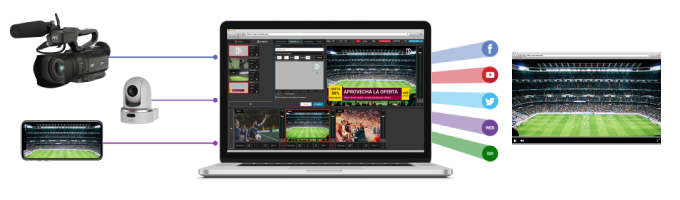
\includegraphics[width=10cm,height=10cm,keepaspectratio]{images/FrontendMixer}
\par\end{centering}
\caption{Frontend Mixer\label{fig:Frontend-Mixer}}

\end{figure}

A partir d'això, es treu un streaming de output en WebRTC RTP, que
es pot emetre automàticament a tots els llocs que el client desitji
(Facebook, Youtube, Instagram, etc.)

En quant al backend, s'ocupa de realitzar les tasques demanades desde
el frontend explicat anteriorment. A més de controlar les diferents
configuracions com poden ser la transcodificació dels videos, configuració
dels videos...\\

\textbf{Parts a substituïr}\\

Encara que hi han alguns elements que primera vista poden semblar
que es poden reutilitzar, no és així, ja que la idea es canviar totalment
el sistema desde la base, utilitzant un altre tipus de software totalment
diferent, veient que l'actual està molt limitat. Per tant, s'ha decidit
no utilitzar res de l'anterior projecte i crear-ho tot desde zero.\\

\subsubsection{Requeriments del nou Mixer}

Per crear el nou Mixer s'han definit una sèrie de requisits que ha
de tenir, per tal de que compleixi amb les expectatives i sigui útil
per duur a terme aquesta ``evolució''. És possible que el producte
final acabi tenint més funcionalitats de les que s'esmenten a continuació,
però sí que reflexa les més bàsiques que ha de tenir.
\begin{itemize}
\item Serà necessari que es puguin definir \textbf{escenes}, les quals també
puguin emmagatzemar les posicions dels elements dins de cada una i
totes les seves propietats.
\item Poder injectar un \textbf{flux d'streaming}
\item Poder injectar un video \textbf{pre-enregistrat (local)}
\item Tot tipus d'elements s'han de poder insertar amb \textbf{posicions
i paràmtetres inicials}
\item Injecció d'\textbf{imatges} amb transparència, a més de permetre el
canal \textbf{alpha}
\item Possibiltat de tenir fins a \textbf{6 fonts }d'streaming \textbf{simultàniament}
\item Els flux d'entrada poden tenir \textbf{diferents resolucions}
\item Extreure el render final via streaming (\textbf{rtp} o similar)
\item Poder definir la resolució i framerate del render final (720p/25fps,
720p/30fps, 1080p/30fps, etc.)
\item Poder canviar d'un element a un altre tant per \textbf{tall} com per
\textbf{dissolve}
\item \textbf{Mute}/unmute de cada font d'entrada
\item Control de volum de cada font d'entrada
\item Mixing de les fonts no mutejades
\item Control de volum de la sortida mesclada
\item Mute/unmute de la sortida mesclada
\item \textbf{Chroma-keying} a les fonts de video (streams o local)
\item Possibilitat de treballar fins a \textbf{4K}
\end{itemize}
\subsection{Eines Gràfiques}

\subsubsection{Headless Chrome}

\textbf{Vanilla}\\

La primera opció que es va proposar va ser utilitzar Headless Chrome.
A partir de la versió 59 de Chrome (actualment està per la versió
90), és possible executar-lo de manera \textit{headless}, el que significa
que es pot utilitzar desde terminal, o més interesant, desde un servidor
sense cap tipus de UI. Es va crear pensant en que podria ser molt
útil, per fer testos automatitzats de webs o aplicacions online.\\
Per executar-lo és molt fàcil, només cal afegir uns quants paràmetres
d'inici al Chrome. Els paràmetres d'exemple són:\\

\lstinputlisting[breaklines=true,captionpos=b,frame=tb,language=bash,caption={Config Headless Chrome},label={chrome}]{code/hchromeconf_1.txt}

Encara que està pensat per fer automatitzacions com he comentat abans,
es pot aprofitar la potència de Chrome per altres tasques, com poden
ser la reproducció de videos, crides a APIs, entre altres.

Buscant algun exemple per internet que aprofités Headless Chrome per
la reproducció de video, ens vam trobar amb uns quants que havien
pensat el mateix.

En un article \cite{HeadlessChromeExp1} trobem que van aconseguir
fer streaming a Facebook i Youtube Live amb uns resultats bastant
satisfactoris. A partir d'una web (video + àudio), ho convertien a
un flux de sortida RTMP. Comenta que el més complicat va ser aconseguir
que el video i l'àudio estiguessin sincronitzats. Però finalment ho
va aconseguir gràcies al controlador d'àudio anomenat PulseAudio \cite{PulseAudio}.

Headless Chrome està pensat per ser utilitzat amb alguna eina d'automatització,
i així ho recomanen desde el propi blog oficial de Google Developers
\cite{HeadlessChromeDevel}. Degut a que no disposem de cap tipus
de UI per debugar o interactuar, utilitzarem una eina externa. Al
blog de Google ens parlen de Puppeteer, Selenium, WebDriver i ChromeDriver.
Totes elles tenen el mateix objectiu, automatitzar tasques al navegador.
Podriem dir que la més desenvolupada i consolidada, és Selenium, però
Pupeteer també s'ha guanyat molt de renom en els últims temps, per
tant, haurem de fer un estudi per veure els pros i contres de cada
una i decidir amb quina d'aquestes ens quedarem.\\

\textbf{Selenium}\\
 

Selenium és una eina gratuïta i open-source \cite{Selenium}, que
serveix per crear tasques automatitzades en un navegador o aplicació
per validar funcionalitats. Es poden utilitzar scripts tant de C\#,
Python, JavaScript, PHP, Scala... Realment Selenium com a tal és una
Suite que es composa d'un grup d'eines; el seu propi IDE, Grid i WebDriver.
Nosaltres estem interessats en l'últim, per tant és el que estudiarem.\\

Selenium WebDriver pot controlar un navegador tal i com ho faria un
usuari, ja sigui de manera local o remota en un servidor. 

\begin{figure}[H]
\begin{centering}
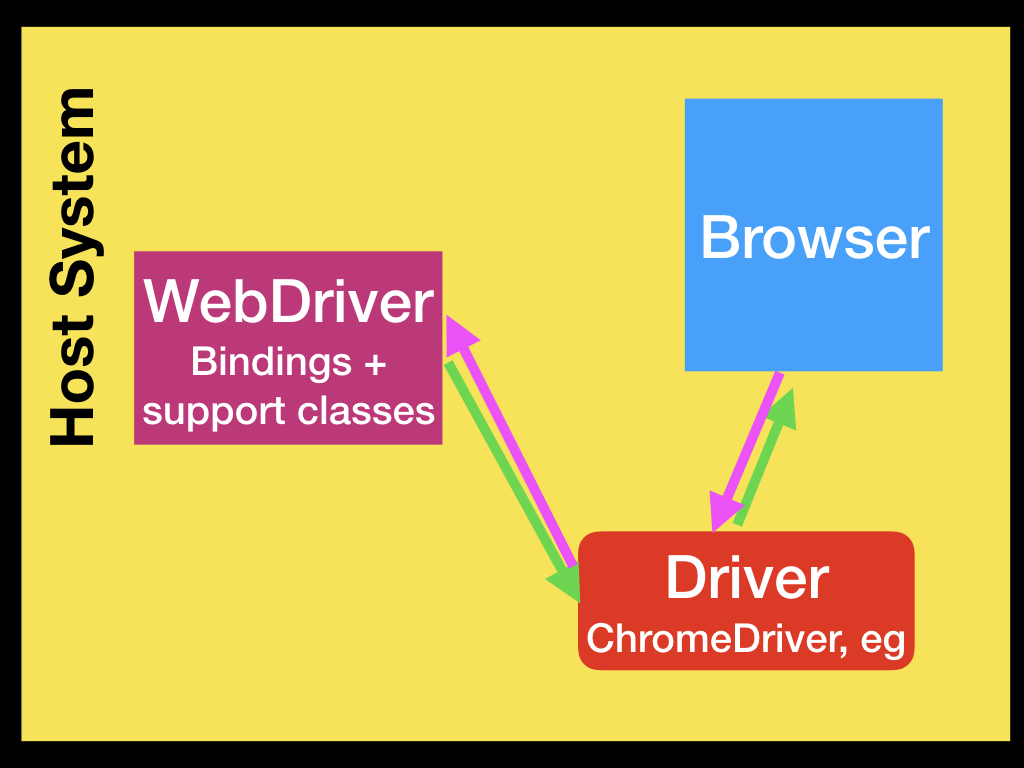
\includegraphics[height=5cm]{images/SeleniumGraph}
\par\end{centering}
\caption{Selenium Driver Graph\label{fig:Selenium-Graph}}
\end{figure}

Com podem veure a la figura \ref{fig:Selenium-Graph}, WebDriver es
comunica amb el navegador a través d'un driver. Aquest driver és específic
de cada navegador. El que ens interessa és el de Chrome, per tant
sabem que utilitzarem el ChromeDriver.\\

Els navegadors que suporta són: Chrome, Chromium, Firefox, Internet
Explorer, Opera i Safari. A la seva documentació \cite{SeleniumDriverDocumentation}
no comenten en cap lloc compatibilitat amb Headless Chrome, però degut
a que està basat en el propi navegador, i no fa cap canvi brusc en
el seu funcionament, podem assegurar que també serà compatible. Ho
podem corroborar amb un article on ho experimenta \cite{SeleniumHeadlessChrome},
en el que expliquen que només hem d'indicar el driver corresponent
a Chrome, i escriure a les opcions, el flag <<--headless>>.\\

\textbf{Puppeteer}\\

Per altre banda tenim un altre eina bastant més nova, anomenada Puppeteer
\cite{Puppeteer}. Les funcionalitats principals venen a ser molt
semblants a Selenium, controlar totes aquelles coses que podries fer
manualment al navegador, fer-ho de manera automàtica. A més de funcionalitats
molt útils com fer captures de pantalla i crear PDFs.\\
\begin{figure}[H]
\begin{centering}
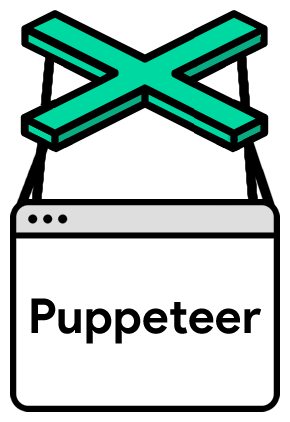
\includegraphics[height=5cm]{images/pupeteer}
\par\end{centering}
\caption{Pupeteer Logo\label{fig:PupeteerLogo}}
\end{figure}

És open source i està sota la llicència d'Apache 2.0 \cite{ApacheLicense}
pel que es pot utilitzar i comercialitzar de manera totalment lliure
tot aquell contingut que tingui les seves eines.

És molt fàcil d'instalar, ja que només cal instalar un paquet npm
i per utilitzar-lo es fa tot amb javascript mitjançant les comandes
que disposen a la seva documentació. A més de tot això, la major ventatja
que té és que està pensat per ser utilitzat amb Headless Chrome, dóna
moltes facilitats per realitzar totes les tasques sense estar veient
cap tipus de UI, i a la vegada poder debuggar de manera còmode i senzilla.
\\

Un petit codi d'exemple que ens mostren a la seva documentació per
comprovar com de fàcil és utilitzar-lo. El que fem és afegir puppeteer
al nostre script de js amb require, iniciem el navegador en mode headless,
obrim el link <<https://example.com>>, fem una captura i tanquem
el navegador. 

\lstinputlisting[breaklines=true,captionpos=b,frame=tb,language=Java,caption={Puppeteer Get Started Example},label={puppeteer}]{code/puppeteerExample_1.txt}

\subsubsection{WebGL Headless}

WebGL és una API escrita en Javascript utilitzada per la renderització
de gràfics en 3D al navegador. Està basat en la Open Graphics Library
(OpenGL), pel que només necessitarem que sigui compatible amb aquest
\cite{WebGLBrowserSupport}, sense cap altre dependència que podria
dificultar la compatibilitat. Hem de tenir en compte que encara que
el navegador sigui compatible, per tota la renderització 3D, per molt
mínima que sigui, necessitarem una targeta gràfica, Això pot ser un
problema ja que es vol executar tot en un model cloud, al donar estabilitat
i professionalitat. La majoria de gent que utilitza servidors té unes
idees bastant diferents al que es vol fer aquí, i potser necessiten
potència de CPU o molta RAM, però no GPU, pel que potser és complicat
trobar una màquina remota amb la potència suficient que es necessita.\\

\begin{figure}[H]
\begin{centering}
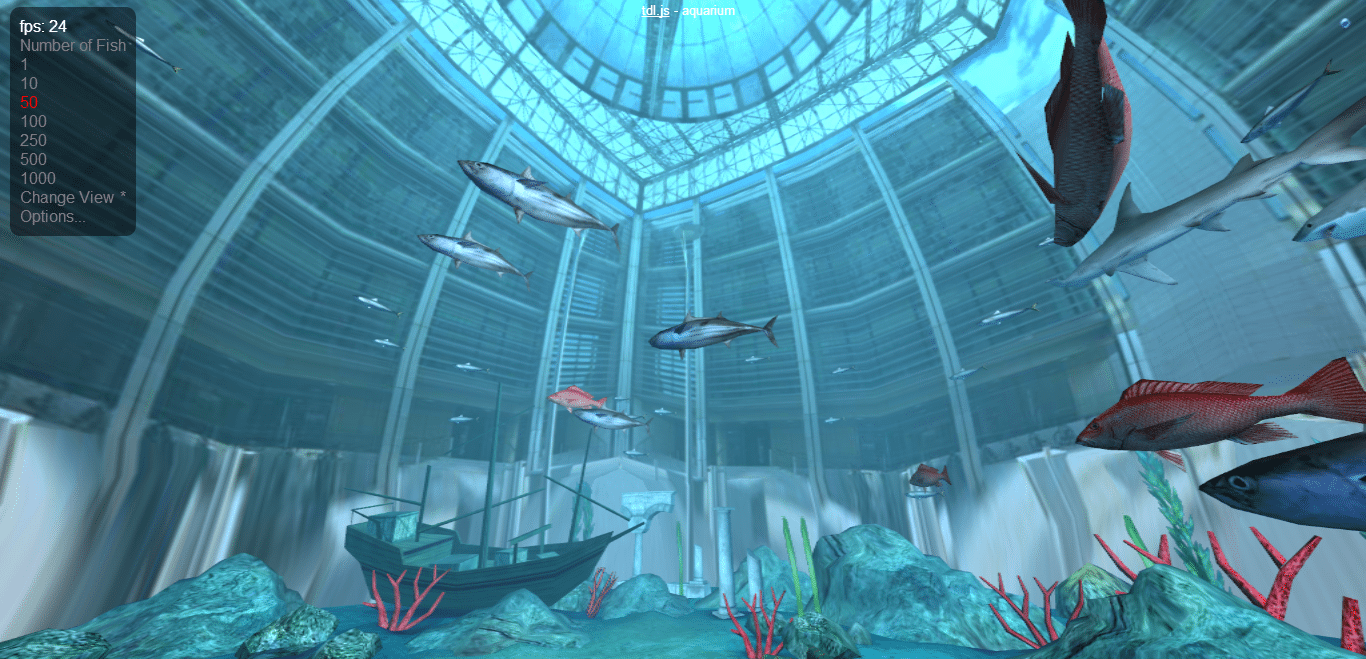
\includegraphics[height=5cm]{images/WebGLAquarium}
\par\end{centering}
\caption{Exemple WebGL\label{fig:WebGLExample}}
\end{figure}

Per una banda aquesta solució és molt atractiva ja que es faria tot
el sistema desde 0 sense utilitzar cap tipus de dependència, però
a la vegada també depens de les polítiques o limitacions de potència
del navegador. Mai serà capaç d'utilitzar el 100\% de la màquina i
no és comparable amb una aplicació standalone.

\subsubsection{Unreal Engine 4}

Un dels motors gràfics més utilitzats dels últims temps és Unreal
Engine. Està creat per Epic Games, programat en C++ i amb una potència
sorprenent que fa que sigui el més utilitzats en projectes fotorrealistes,
o inclús, en projectes d'arquitectura. Sobretot a partir de 2019,
on van juntar-se amb l'empresa Quixel, dedicada entre d'altres coses,
a crear <<megascans>>. És una tecnologia que diposa textures amb
grans resolucions i qualitats sorprenents, però a la vegada molt eficients
pel desenvolupament de videojocs. Així aconseguint un renderitzat
molt realista a temps real, i destacant entre els altres motors competidors.

\begin{figure}[H]
\begin{centering}
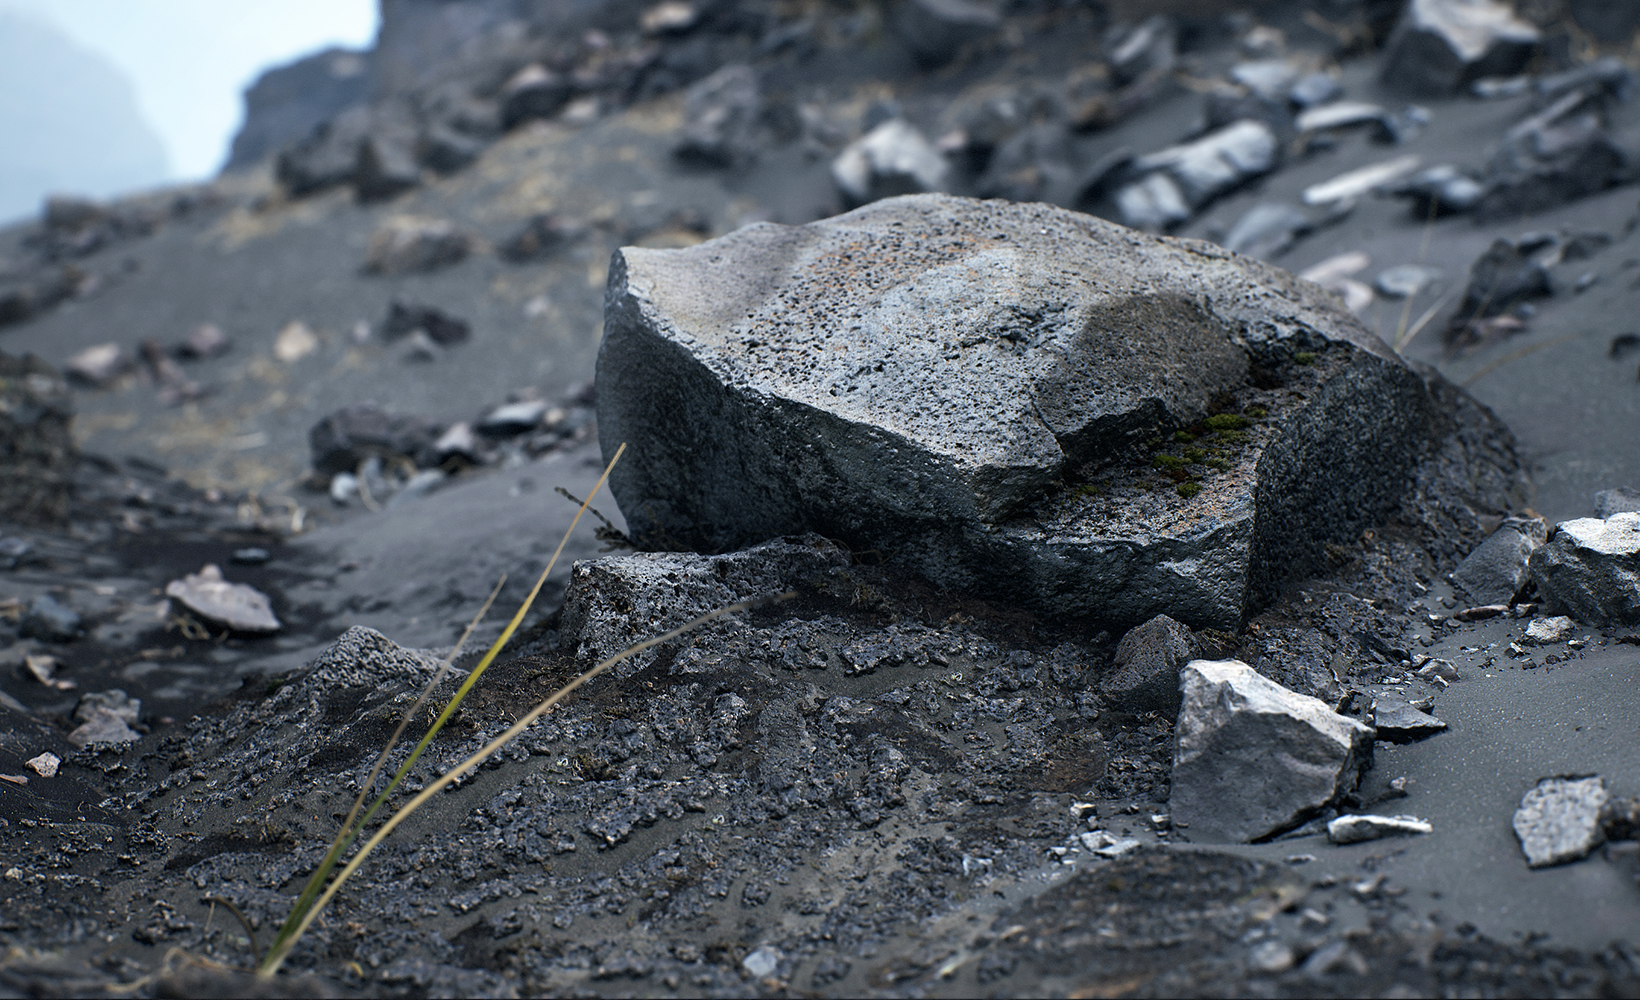
\includegraphics[height=5cm]{images/Quixel}
\par\end{centering}
\caption{Captura Quixel Demo Megascan a UE4 (Youtube)\label{fig:QuixelMegascans}}
\end{figure}

Durant el transcurs del 2021 es llençarà la versió d'Unreal Engine
5, on han demostrat que poden inclús superar-se i crear uns entorns
sorprenents juntant la tecnologia que ja havien estat desenvolupant
de Quixel, amb una nova anomenada Lumen, que controlarà totes les
llums i farà ús del Ray-Tracing a temps real, també dit RTX a les
targetes gràfiques de Nvidia. Amb totes aquestes novetats i evolucions
tecnològiques que han anat fent en els últims anys, és lògic que s'hagin
guanyat entre la comunitat el nom a millor motor gràfic en quant a
qualitat visual \cite{UE4BestPhotoEngine}. Però com bé sabem, això
no és l'únic que importa.\\

L'Unreal disposa d'un sistema de programació anomenat Blueprints,
és una metodologia de programació totalment visual i basada en nodes.
Bàsicament són petites capces que internament tenen trossos de codi
en C++, els quals juntem entrades i sortides.

\begin{figure}[H]
\begin{centering}
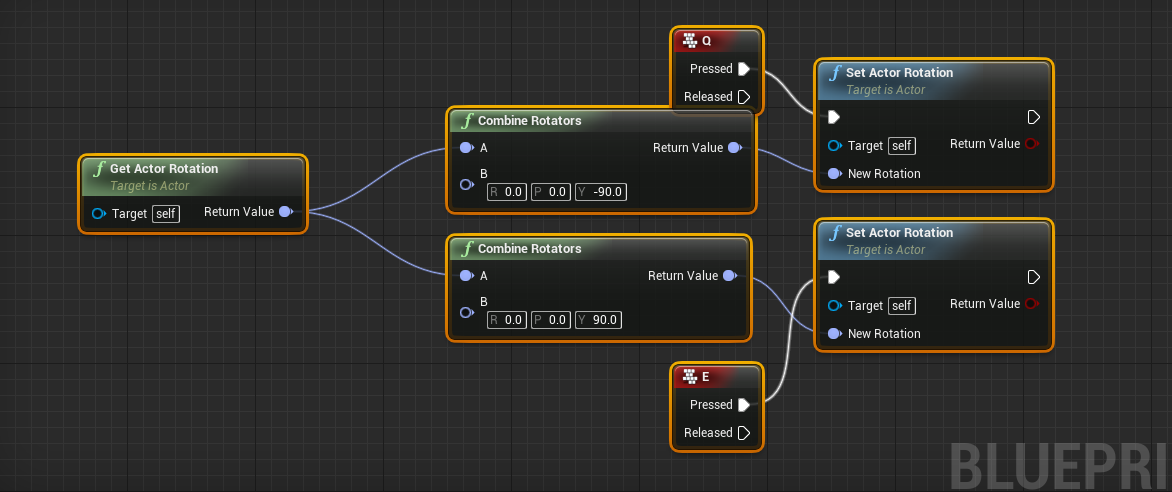
\includegraphics[height=5cm]{images/BlueprintRotate}
\par\end{centering}
\caption{Rotació Programada en Blueprint UE4\label{fig:BlueprintRotate}}
\end{figure}

Això pot ser molt còmode i és un punt a favor per la gent que comença
a desenvolupar videojocs, si estàs acostumat a utilitzar-ho o no es
tenen els coneixements necessaris de programació i vols fer scripts
amb una complexitat baixa-mitjana. Però pel contrari si es volen fer
scripts més complexes pot ser que ens trobem amb certs inconvenients
i poden quedar scripts amb milers de nodes i que sigui molt difícil
d'interpretar o debugar.

\begin{figure}[H]
\begin{centering}
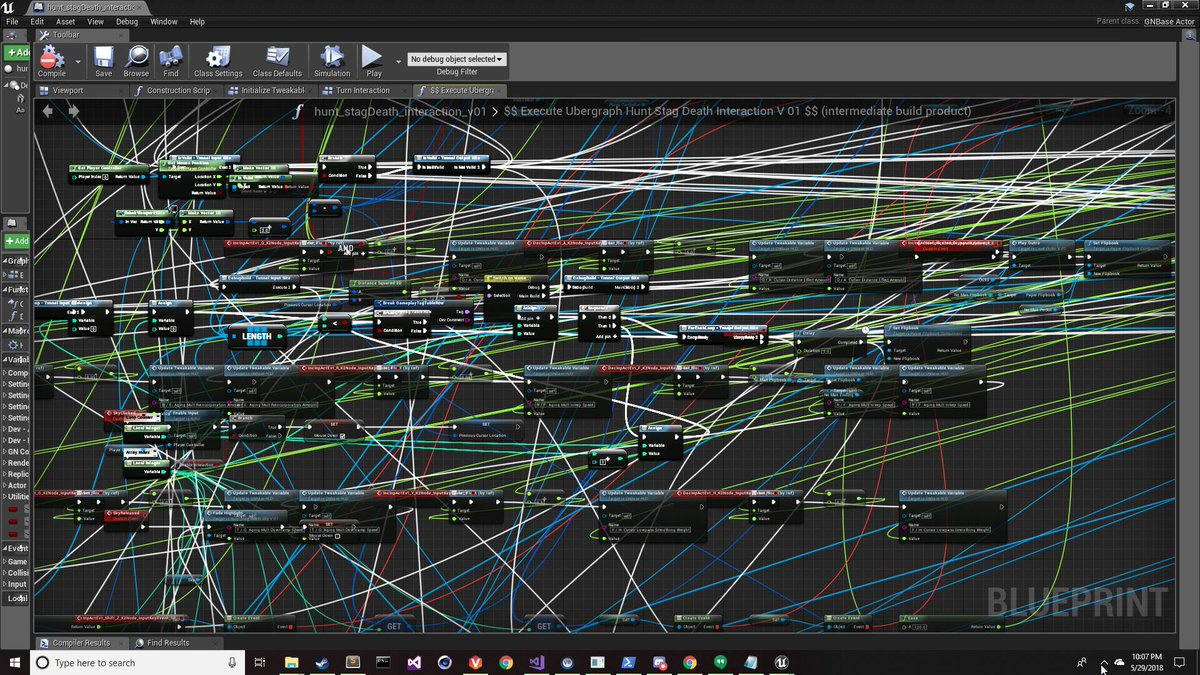
\includegraphics[viewport=0cm 9mm 1200bp 675bp,clip,height=5cm]{images/BlueprintChaos}
\par\end{centering}
\caption{Exemple Blueprint Caòtic UE4\label{fig:BlueprintChaos}}
\end{figure}

Altres inconvenients poden ser que les idees que es tenen surtin fora
de la norma, que els nodes estiguin massa limitats o que simplement
no t'agradi, per això també et donen la opció a crear un script buit
i fer-ho tot amb C++. I llavors veiem que la documentació que es pot
trobar és molt inferior a la dels blueprints, i possiblement sigui
més complicat i més llarg de fer que els seus competidors, com poden
ser Unity o Godot.

\subsubsection{Unity}

El motor de videojocs més famós i més utilitzat desde els seus origens
és sense dubte Unity \cite{PopularUnity}. Va ser creat al 2005 a
Copenhaguen per 3 amics, David Helgason, Joachim Ante i Nicholas Francis.\\

És el motor que suporta més plataformes actualment \cite{UnityMultiplatform},
com Windows, Mac OS, Linux, iOS, Android, WebGL, Playstation, Xbox,
Nintendo Switch, Stadia i moltes altres més. Això és un punt molt
a favor, ja que necessitem desenvolupar l'aplicació per un servidor
Linux, i Unity és el motor més professional dels que donen suport.
Altres motors com Unreal Engine, Game Maker o Cry Engine no accepten
el sistema operatiu Linux com a opció de compilació, o funcionen amb
bastants problemes.\\

La programació dels scripts es fa amb llenguatge C\# el qual forma
part de la plataforma .NET propietaria de Microsoft. És un llenguatge
derivat de C/C++ i és dels més utilitzats juntament amb Java. Si ens
fixem en el rànking de plataforma TIOBE \cite{TIOBE}, que és una
web que s'encarrega d'ordenar els llenguatges de programació de més
utilitzat a menys, podem veure que en el top 5, tenim els 3 llenguatges
de C, els quals tenen una base molt semblant. Després tindriem Java
i Python, tots dos són llenguatges d'alt nivell molt senzills i que
faciliten molt el flux de programació.

\begin{figure}[H]
\begin{centering}
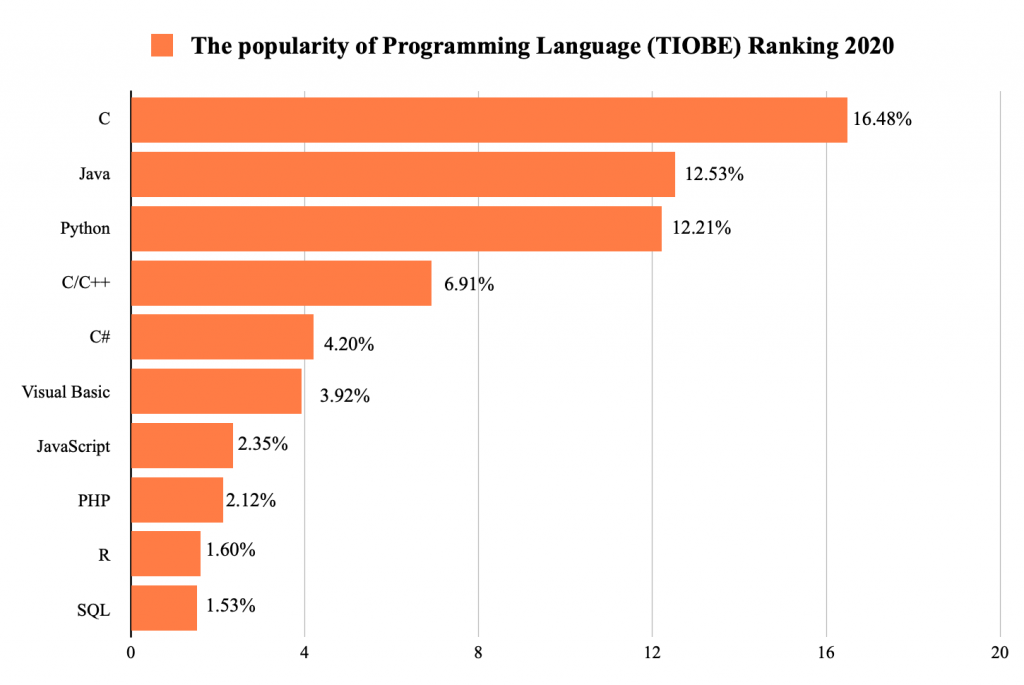
\includegraphics[viewport=0cm 6.75328mm 900bp 506.496bp,clip,height=5cm]{images/RankingLanguages}
\par\end{centering}
\caption{Llenguatges de programació més utilitzats al 2020\label{fig:TiobeRanking}}
\end{figure}

A més de que Unity utilitzi C\# que ja és un llenguatge d'alt nivell
de per si, s'utilitza la API MonoBehaviour \cite{MonoBehaviour},
que estalvia molta feina i permet fer tasques que a priori són complicades
o llargues, en pocs minuts i en poques linies.

MonoBehaviour és la classe base d'on parteixen tots els scripts de
Unity. Només cal indicar que el nou script s'extén de la API.\\

\lstinputlisting[breaklines=true,captionpos=b,frame=tb,language={[Sharp]C},caption={Unity Code Basic Template},label={unitytemplate}]{code/UnityCode.txt}

En les últimes versions de Unity, han apostat molt per competir directament
amb Unreal Engine, en un dels punts que tenien més diferenciats, l'atractiu
visual hiperrealista.

Quan Unity va començar, com que era relativament fàcil d'utilitzar
i gratis, van aparèixer una quantitat immensa de jocs de mòbil creats
amb aquest motor, pel que es va guanyar una fama errònea, de que aquest
motor només servia per jocs petits, amb uns gràfics tirant a simples
i sense molts efectes. 

Per tant, al 2019 van llençar amb la seva última actualització, una
nova funció anomenada HDRP (High Definition Render Pipeline) \cite{HDRP},
la qual millorava tot el sistema del render del motor, aconseguint
uns resultats que van sorprendre a tota la comunitat, i que no tenien
res a envejar amb Unreal Engine.

\begin{figure}[H]
\begin{centering}
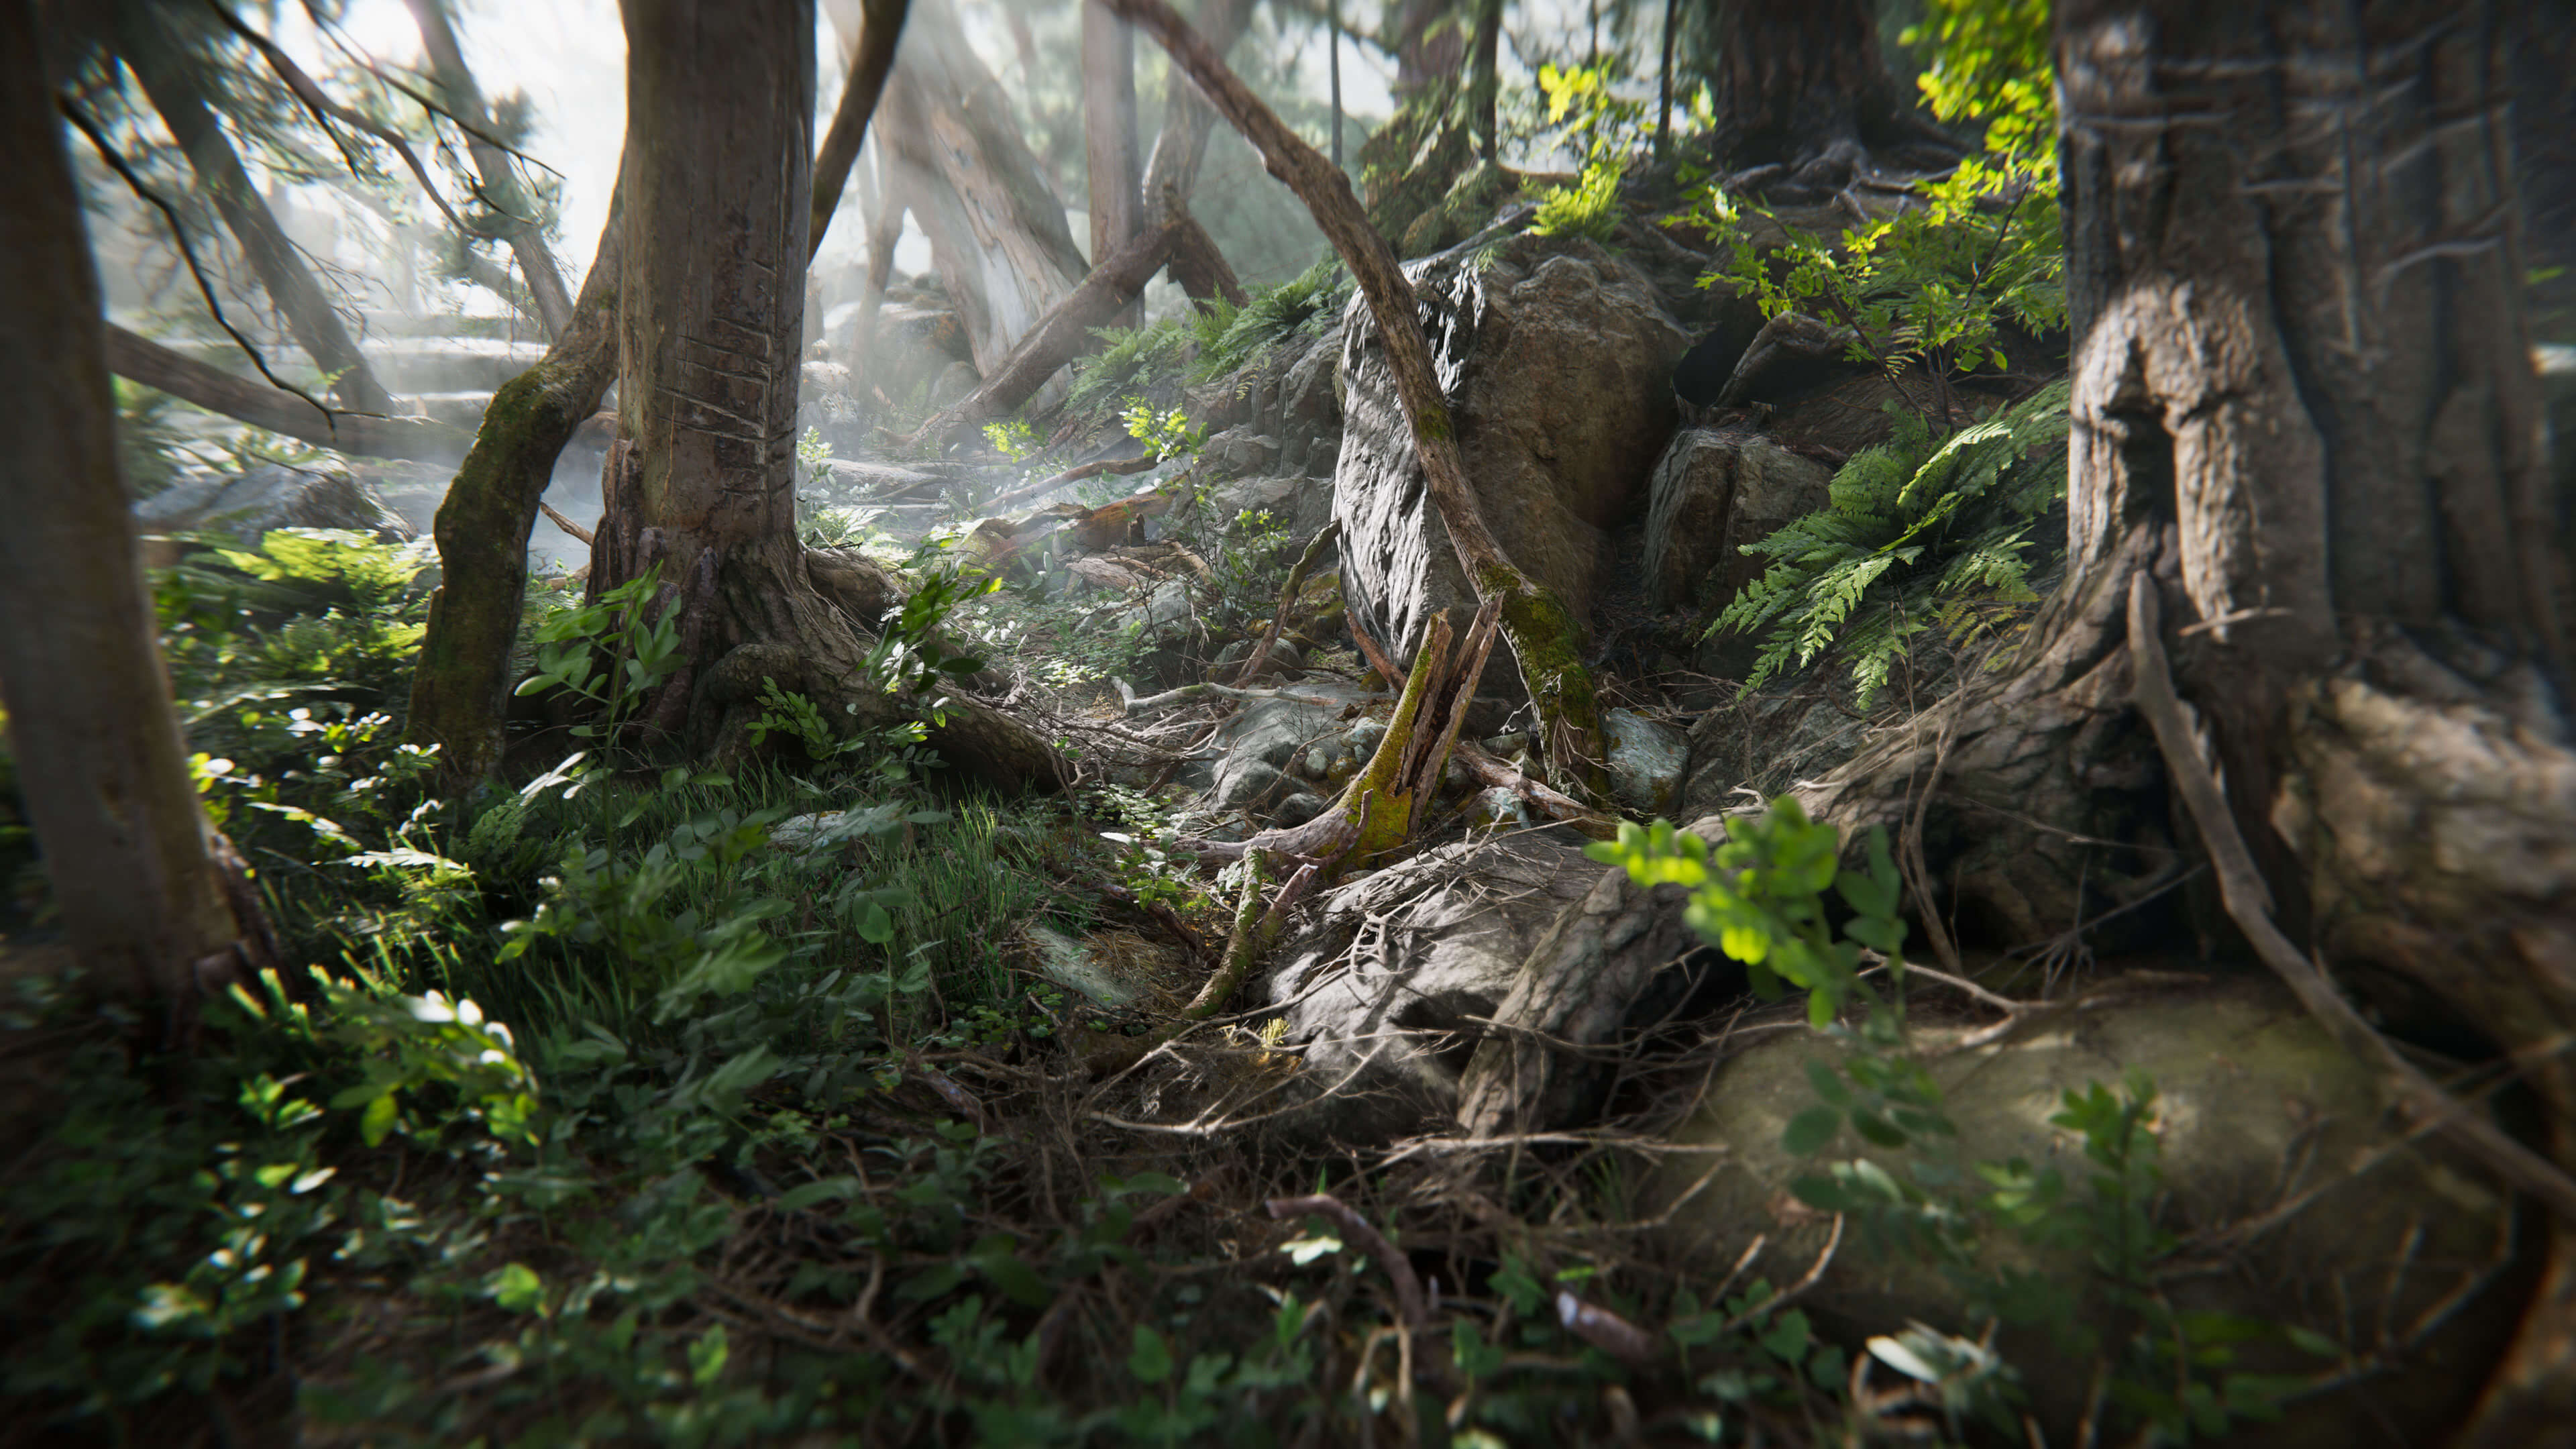
\includegraphics[height=5cm]{images/UnityPhotorealism}
\par\end{centering}
\caption{Captura Book of the Dead Unity Demo HDRP (Youtube)\label{fig:BookOfDead}}
\end{figure}

A més, podem trobar que el videojoc més realista que s'ha creat mai
en quant al gènere de FPS (First Person Shooter), van decidir crear-lo
amb el motor Unity, enlloc d'Unreal, i van aconseguir uns resultats
molt bons, fins al punt que està considerat el joc amb millors gràfics,
creat amb aquest motor. Es tracta del videojoc \textit{Escape from
Tarkov}.

\begin{figure}[H]
\begin{centering}
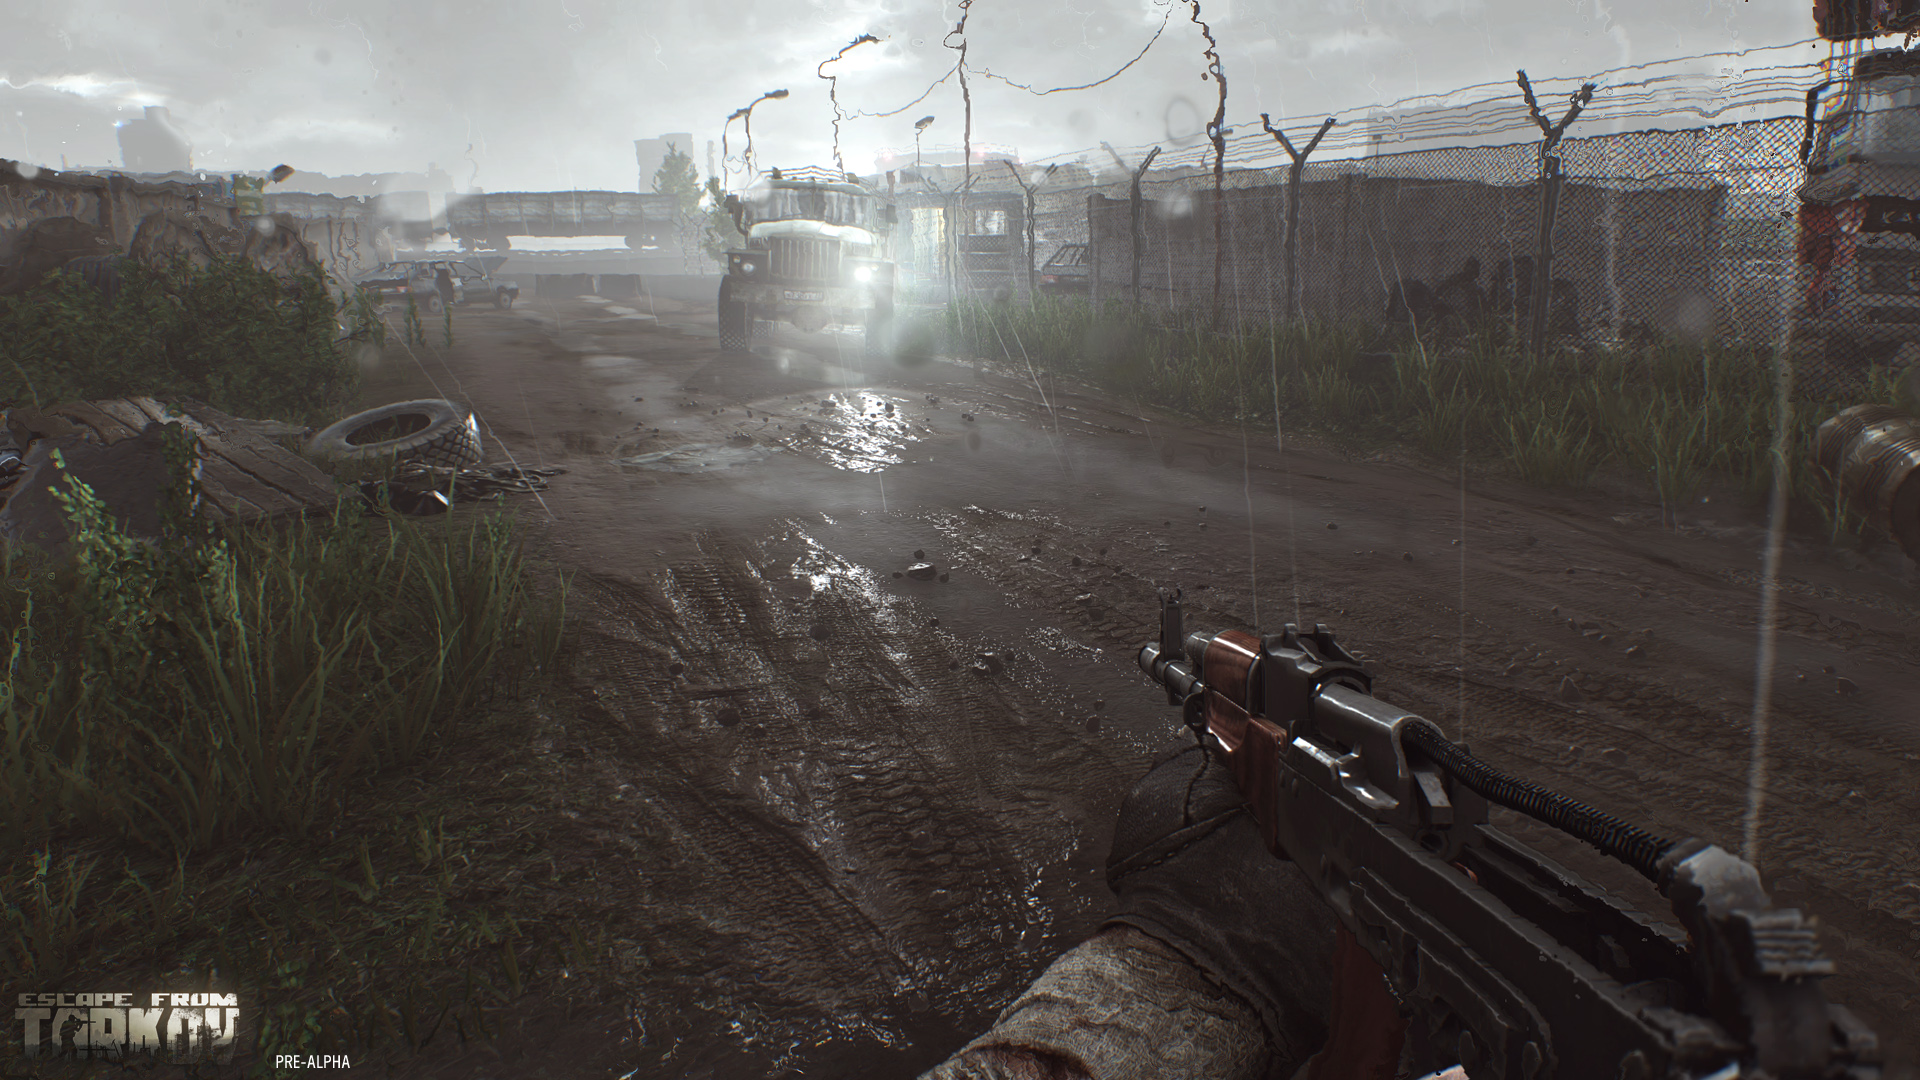
\includegraphics[height=5cm]{images/eft}
\par\end{centering}
\caption{Captura Escape from Tarkov Pre-Alpha\label{fig:EFTCaptura}}
\end{figure}

\subsection{Tractament dels fluxes de video}

\subsubsection{Formats Compatibles}

L'aplicació haurà de rebre tot tipus de videos, de tots els formats
possibles, entenent formats el conjunt de códecs i contenidors. Primer
s'ha de fer un anàlisi dels formats que existeixen i com de populars
són\textbf{.}\\

\textbf{Códecs}\\

Hi ha molts tipus de códecs, però és cert que alguns s'utilitzen molt
poc, o ja s'han quedat antiquats.
\begin{itemize}
\item H.261: Aquest códec va ser el primer que es va tornar popular, degut
a que era el que donava millors resultats en el seu moment. Però evidentment,
ha passat molt temps i la tecnologia ha evolucionat suficient com
per deixar aquest códec antiquat.
\item H.263: Va ser el primer que códec realment eficient, però a la vegada
demanava molts recursos de l'ordinador per codificar un video, i a
la vegada, per reproduir-lo necessitarem una potencia relativament
alta.
\item H.264: És el més popular a l'actualitat de manera professional, també
conegut com MPEG-4 AVC, compta amb una compressió molt alta amb una
pèrdua de qualitat imperceptible. A més de ser molt polivalent al
acceptar molts tipus de bitrate d'entrada.
\item H.265: També anomenat HEVC, és el successor del H.264. A vegades pot
donar uns resultats pitjors al seu predecessor, però sobretot pels
videos en 4K obtenim uns molts millors resultats ja que comprimeix
molt més obtenint uns resultats de qualitat molt semblants. En els
videos 4K es pot obtenir fins a un 64\% de reducció de bitrate en
comparació amb H.264.
\item MPEG-1: És un códec bastant antic que ja no s'utilitza, però va ser
molt utilitzat per discs de dades CD-ROM i inclou compressió tant
de video com d'àudio.
\item MPEG-2: Dona bons resultats amb el DVD, però requereix pagar llicència
per poder-lo utilitzar.
\item MPEG-4: S'utilitza molt per contigut de videos a la xarxa, ja que
té una gran compressió de vídeo i àudio, però la qualitat pot baixar
al utilitzar baixos nivells de bitrate.
\item X264: Molt similar al H.264 amb la gran diferència de ser open-source,
el que fa que sigui el més utilitzat de manera gratuita, amb els millors
resultats.
\item DivX: Comunament utilitzat per comprimir películes DVD i famós per
impulsar la pirateria al voltant de l'any 2000 al permetre comprimir
fins a 7 pelicules en un sol disc DVD \cite{DivX}.
\end{itemize}
%
\textbf{Contenidors}\\

\begin{itemize}
\item AVI: Cada cop és menys utilitzat, però a l'anterioritat va ser molt
popular per la gran compatibilitat de la que disposava en diferents
sistemes operatius.
\item MOV: A diferència de l'AVI, aquest códec creat per Apple, era molt
poc o gens compatible amb altres sistemes operatius, pel que només
s'utilitzava amb els seus dispositius.
\item MPG: Són un conjunt de formats, i alguns d'ells han arribat a ser
els més famosos, sobretot el MPG-4, també anomenat MP4. Que té molta
qualitat, comparable al MOV, i actualment és pràcticament impossible
trobar algun ordinador que no sigui capaç de reproduir-lo.
\item WMV: Windows Media Video és un format propietari de Windows, i necessitarem
reproduir-lo amb el Windows Media Player per aconseguir els millors
resultats d'aquest.
\item MKV: Acrònim de Matroska, és un format molt utilitzat per emmagatzemar
més d'un arxiu en un sol. Per exemple podem trobar un arxiu MKV que
contingui més d'una pista d'àudio (per diferents idiomes), alguns
arxius de subtítols o inclús diferents arxius de video en un sol.
\item FLV: El format de video de Flash Player, que és molt compatible amb
tots els ordinadors, però cada cop s'està quedant més antiquat.
\end{itemize}
%
Els reproductors més famosos, com són VLC, MPV, o MPlayer, accepten
tots els tipus de códecs i contenidors, pel que serà necessari i pràcticament
requisit que l'aplicació també els accepti tots per a que no es quedi
enrera. Ja sigui creant un reproductor propi, o un basat en llibreries
de tercers.\\

\textbf{Imatges}\\

En quant a les imatges, també trobem molts formats diferents i s'haurà
de tenir en compte per decidir si es podrà donar suport a tots ells,
o pel contrari s'haurà de prescindir d'algun. Com a mínim hauria d'acceptar
els més famosos, que són:
\begin{itemize}
\item BMP: Creat per l'empresa Microsoft, és l'estàndard del sistema operatiu
Windows.
\item JPEG: Un dels formats més utilitzat degut a la seva gran compressió,
mantenint una qualitat molt acceptable.
\item GIF: El GIF és un format diferent a la resta, ja que consta d'un conjunt
d'imatges que es reprodueixen de manera continua, formant un petit
video. Això si, la seva qualitat queda molt limitada.
\item PNG: Disposa d'una gran compressió mantenint la qualitat, com podria
ser la del JPEG, però, amb la gran ventatja de que disposem de l'atribut
alpha, el que permet tenir imatges amb transparències.
\end{itemize}
%
\textbf{Àudio}\\

Els videos tindràn el seu propi àudio, i encara que no està pensat
com a requisit que es pugui reproduir àudio de manera independent,
com podria ser una música de fons o una veu en off. Els formats que
s'haurien de suportar per poder tenir un mínim de compatibilitat són:
\begin{itemize}
\item WAV: Desenvolupat per Microsoft i un dels més utilitzats, és compatible
amb pràcticament tots els códecs. Accepten arxius d'un tamany gran
fins a 4GB, i poden estar molt comprimits o poc.
\item MPEG: Un dels formats més famosos per ser un estàndard en àudio i
sobretot, en la música, podem trobar per exemple els códecs MP2 (més
utilitzat per aplicacions de broadcast) o el MP3.
\end{itemize}
%
\subsubsection{Protocols de Streaming}

En quant a la sortida del video/àudio resultant, s'haurà de decidir
quin protocol s'utilitza, ja que es voldrà una sortida en streaming.
El video en streaming, o retransmisió en directe, és la emisió d'un
flux de dades a temps real, o amb el menor retard possible, a un destí.
Per exemple, quan mirem la televisió, tenint en compte que és per
internet i no per antena, estem rebent un flux de dades que arriba
desde uns servidors centrals de la cadena en particular. Es van començar
a fer experiments de televisió fa molts anys, però la majoria van
ser un fracàs degut al gran ample de banda que demanaven els videos.
Per tant el que va sorgir primer van ser els serveis de VOD (Video
on Demand). No s'ha de confondre el VOD amb el Streaming ja que son
dos conceptes totalment diferents i que no utilitzen les mateixes
tecnologies. Un exemple de servei VOD que va triunfar és la plataforma
Youtube. Aquesta tecnologia va anar avançant fins que van millorar
les conexions a internet i això va provocar que per fi el Streaming
fos possible. L'objectiu del directe, és tenir un retard mínim, amb
una qualitat bona. Actualment el mínim de qualitat per una plataforma
professional és la resolució 1920x1080. La resolució 4K dona molt
bona qualitat, però requereix una quantitat molt alta d'ample de banda
i actualment grans plataformes de streaming com Youtube o Twitch no
ho permeten com a opció. Encara i això serà un repte a tenir en compte
i seria un gran punt a favor respecte a la competència.

Els protocols de streaming són els encarregats de posar les <<normes>>
en com es transmetrà el flux de dades, a més de contemplar els errors
i minimitzar-los en tot lo possible.

Un protocol no té res a veure amb un códec o un format, sinó que és
complementari a aquests i només s'ocupa de la transmisió.

\begin{figure}[H]
\begin{centering}
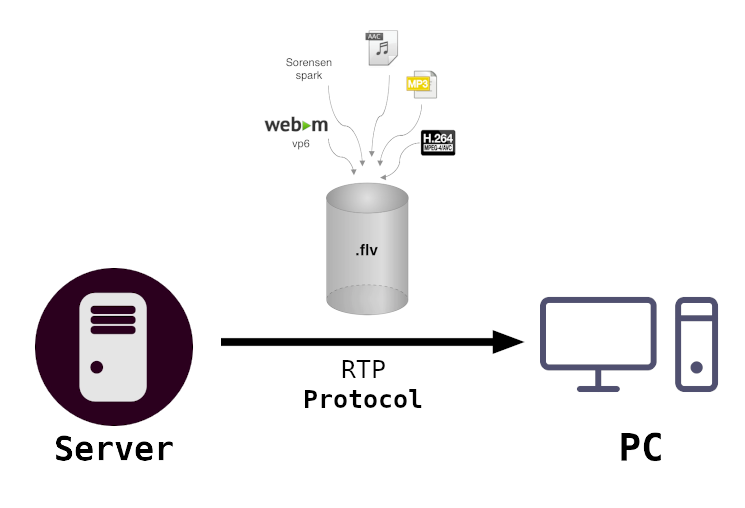
\includegraphics[height=5cm]{images/DiagramaProtocol}
\par\end{centering}
\caption{Diagrama Protocol-Format-Códec\label{fig:DiagramaProtocol}}
\end{figure}

Tots els protocols hauràn d'utilitzar un dels dos mètodes de transmissió
que existeixen, que són TCP (Transmission Control Protocol) o bé,
UDP (User Datagram Protocol). La diferencia més important i notòria
entre aquests, és que el TCP, requereix d'una resposta del client,
forçant a que tots els paquets arribin, el que fa una connexió més
segura, però més lenta. Quan TCP no aconsegueix enviar un paquet correctament,
repeteix el procés fins a aconseguir-ho. Per altre banda, UDP ignora
això, simplement envia els paquets, i el receptor ja s'ocuparà de
rebre-ho correctament. Això provoca que a vegades es puguin percebre
fragments en el video i pèrdua de qualitat, però és molt més ràpid
i té menys retard. 

\begin{figure}[H]
\begin{centering}
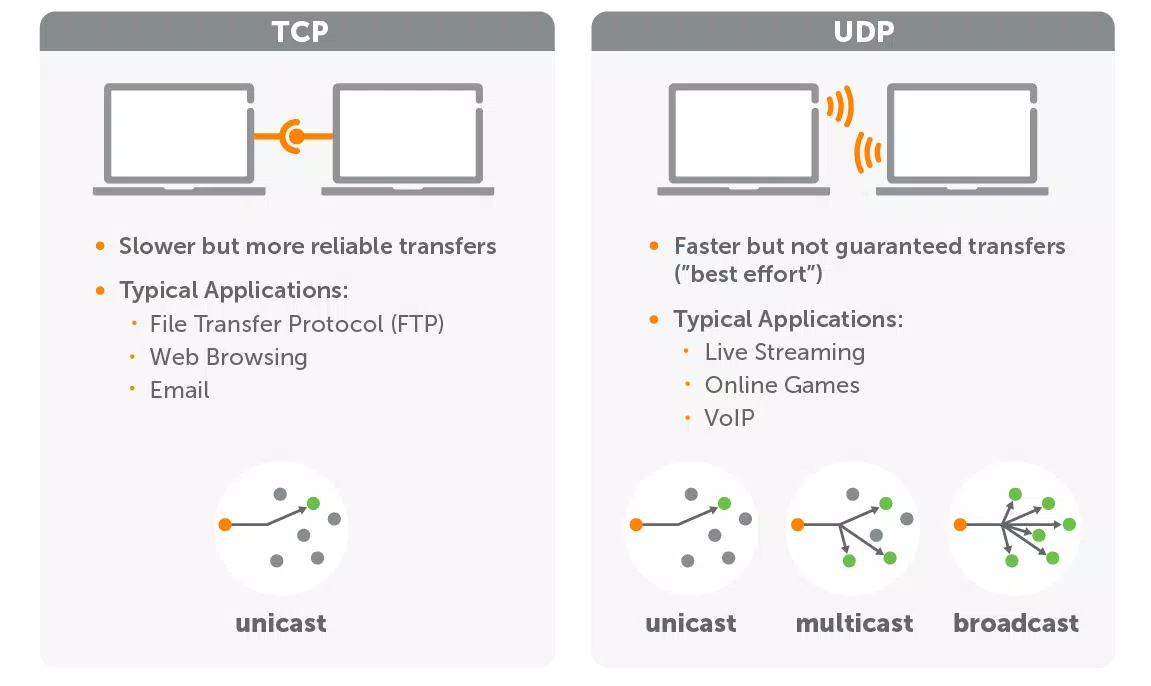
\includegraphics[height=5cm]{images/TCPvsUDP}
\par\end{centering}
\caption{Comparació TCP-UDP\label{fig:TCPvsUDP}}
\end{figure}

Tornant als protocols de live streaming, hi ha molts per escollir,
pel que es comentaran els més importants.
\begin{itemize}
\item RTMP (Real Time Messaging Protocol): Protocol TCP. És propietat d'Adobe,
pel que era molt utilitzat a les webs que disposaven d'Adobe Flash
Player. No obstant, s'ha quedat bastant obsolet i presenta problemes
de compatibilitat amb códecs moderns i la seguritat és baixa. Per
altre banda, els resultats que dona són de bona qualitat i té molt
suport amb les diferents plataformes i software. Els codecs més recomanats
per aquest protocol són H.264 pel video, i AAC per l'àudio.
\item WebRTC: Protocol TCP i UDP. Utilitzat per la gran majoria de desenvolupadors
web, degut a la seva gran compatibilitat amb tots els navegadors moderns:
Chrome, Firefox, Opera, Safari, Edge... És de gran qualitat i soporta
els códecs VP8 i VP9, clarament superiors al H.264 en quant a streaming
de video. Per l'àudio, tenim que WebRTC suporta el códec Opus, gairebé
el més utilitzat per videos en directe. A més, amb la ventatja de
ser open source, el projecte està en una constant evolució, i pròximament
suportarà el códec H.265, i més important encara el AV1, que promet
una gran millora en tots els aspectes \cite{AV1Codec}. Té el millor
resultat de latència, podent arribar a valors menors a 1 segon.
\item FTL (Faster Than Light): Protocol UDP. Creat per l'empresa Microsoft,
dedicat a la plataforma ja extinta Mixer \cite{MixerFTL}. Una proposta
que no va sortir del tot bé, i que pretenia competir directament amb
Twitch \cite{MixerCierre}. Aquest protocol té com a objectiu ser
el més ràpid, com indica el seu nom, per poder comunicar-te amb els
visualitzadors del directe d'una manera pràcticament instantània.
Tenint en compte que Twitch utilitza RTMP, i ho converteix a HLS \cite{TwtichRTMP}
(molt més lent que la proposta de Mixer), no era una mala idea. Encara
i això, Twitch ja era massa gran i estàndard com per poder competir.
\item SRT (Secure Realiable Transport): Protocol UDP. També es un protocol
open-source, al igual que WebRTC, i és considerat com a l'evolució
de RTMP. És de molta qualitat i bastant més estable als anteriors.
Els objectius d'aquest projecte són crear un protocol que transmeti
videos sense soroll al senyal (jitter) i que eviti la pèrdua de paquets.
\end{itemize}
%
\begin{figure}[H]
\begin{centering}
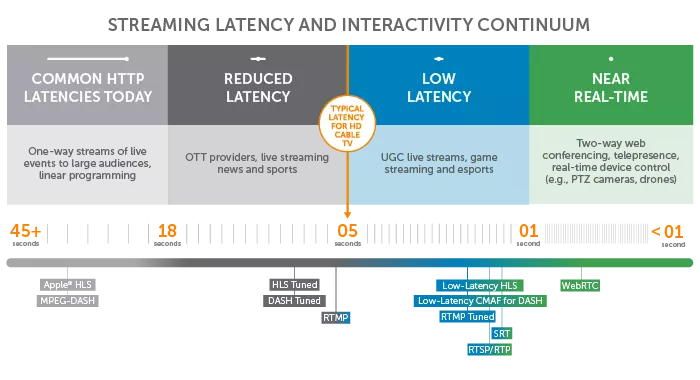
\includegraphics[height=5cm]{images/latencyGraph}
\par\end{centering}
\caption{Gràfic Latències Protocols de Streaming\label{fig:LatencyGraph}}
\end{figure}

Resumint, no hi ha protocols més bons o més dolents, depenent el projecte
que es vulgui fer, serà més adequat un o altre. Pel projecte que s'ha
proposat en aquest treball, es necessitarà sobretot un protocol amb
poc retard.

\begin{table}[H]
\begin{tabular}{|>{\centering}m{2cm}|>{\centering}m{2cm}|>{\centering}m{2cm}|>{\centering}m{2cm}|>{\centering}m{2cm}|}
\cline{2-5} \cline{3-5} \cline{4-5} \cline{5-5} 
\multicolumn{1}{>{\centering}m{2cm}|}{} & \textbf{RTMP} & \textbf{WebRTC} & \textbf{FTL} & \textbf{SRT}\tabularnewline
\hline 
\textbf{Pros} & Estabilitat, gran compatibilitat i qualitat & Open-source, códecs actuals i molt baixa latència & Qualitat adaptativa i molt ràpid & Molta qualitat, estabilitat i compatibilitat de codecs\tabularnewline
\hline 
\textbf{Contres} & Molta latència, més insegur que altres opcions, códecs antics & Constantment en desenvolupament i pot ser inestable & Qualitat inferior a la resta i poca compatibilitat & Està en desenvolupament, no hi ha gaire documentació\tabularnewline
\hline 
\textbf{Video Códecs} & H.264 & VP8, VP9, H.264 (H.265 i AV1 futur proper) & H.264 & -\tabularnewline
\hline 
\textbf{Àudio Códecs} & AAC & Opus & Opus & -\tabularnewline
\hline 
\textbf{Latència} & 3-30 segons & 1 segon o menys & 1 segon o menys (menor a WebRTC) & 1 segon o menys\tabularnewline
\hline 
\end{tabular}

\caption{Taula resum dels protocols esmentats}

\end{table}

\subsubsection{Llibreries de processament}

La gran majoria d'aplicacions que utilitzem a diari que disposen de
reproductors multimedia, o qualsevol tipus de processament de video/àudio,
utilitzen llibreries externes per fer aquest procés més senzill. Hi
ha varies opcions de llibreries de processament de contingut multimèdia.
Totes elles tenen un desenvolupament complex, és per això que hi ha
poca rivalitat, i totes disposen d'una API per utilitzar-les. Les
més utilitzades i conegudes, són dues que es comentaran a continuació:\\

\textbf{FFMPEG}\\

És la llibreria de processament de video/àudio més gran que existeix,
i és utilitzada per la gran majoria de desenvolupadors. 

\begin{figure}[H]
\begin{centering}

\includegraphics[height=2cm]{images/FFmpegLogo}
\par\end{centering}
\caption{Logo FFmpeg\label{fig:FFmpeg}}
\end{figure}

Concretament, el que defineix FFmpeg, és un conjunt de software lliure
(framework), que tal i com diu a la seva documentació \cite{FFmpeg About},
les funcionalitats que permet són: 
\begin{itemize}
\item Decodificar: és l'acció de convertir un flux de dades en un contingut
multimedia visible i amb sentit per a un receptor.
\item Codificar: és l'acció contraria a decodificar, convertir un contingut
multimedia a un flux de dades, ja sigui per una transmissió més còmode,
comprimir, o el que es desitji.
\item Transcodificar: significa convertir un contingut multimèdia d'un códec
a un altre. Per exemple, ens podem trobar amb un contingut en H.265,
que el volem reproduir en un ordinador relativament antic, que no
accepta aquest códec, pel que haurem de transcodificar-lo a un altre
que l'ordinador si que <<entengui>> com podria ser el H.264.
\item Multiplexar: si tenim video i àudio per separat i ho volem juntar,
el que haurem de fer es un mux, és a dir, juntar dos o més fluxes
d'entrada, en un de sortida.
\item Demultiplexar: és el contrari de multiplexar, tenint un sol flux d'entrada,
extreiem dos o més.
\item Stream: si enlloc de voler generar un fitxer de sortida, el que volem
és directament crear un streaming, utilitzant el protocol més apropiat,
ho podem fer tot desde ffmpeg i sense utilitzar cap eina externa.
\item Filtres: per si totes les funcionalitats anteriors fóssin poques,
també permeten aplicar filtres als àudios o als videos, el que ho
fà molt còmode per poder automatitzar tasques desde terminal, sense
haver d'utilitzar editors de video o àudio. En quant a filtres d'àudio
disposem de 105 efectes, entre ells els més senzills com el volum,
compressors... I en quant al video, disposem de 264 efectes, com per
exemple, fer un crop, escalar, rotar... \cite{FFmpeg Filters}
\item Reproduir: FFmpeg també inclou una eina anomenada FFplay, que permet
reproduir tot tipus d'arxius sense problemes. Normalment s'utilitza
com a eina de test.
\end{itemize}
%
Es va desenvolupar principalment per GNU/Linux, però està disponible
per tot tipus de plataformes com Windows i MacOS. S'utilitza a través
d'un terminal, però també es pot integrar en tot tipus d'aplicacions
per utilitzar-lo internament, com fa Audacity, Youtube, Chrome, OBS
Studio, i molts altres grans projectes.\\

\lstinputlisting[breaklines=true,captionpos=b,frame=tb,language=bash,caption={Exemple Transcodificació Arxiu H.265 a H.264},label={ffmpegTranscode}]{code/ffmpegTranscode.txt}

La instalació d'aquesta eina és molt senzilla, sobretot si s'utilitza
Linux, o concretament Ubuntu, es pot aconseguir introduint un parell
de línies al terminal.\\

\lstinputlisting[breaklines=true,captionpos=b,frame=tb,language=bash,caption={Instalació FFmpeg Ubuntu},label={ffmpegInstall}]{code/ffmpegInstall.txt}

També és molt utilitzat per la compressió de videos de manera automàtica,
per exemple, si pujem un video a <<Twitter>>, no es pujarà el video
original, ja que el pes de l'arxiu seria excessiu per emmagatzemar-ho
al seus servidors, sinó que es fa una copia reduida del video, i aquest
és el que es guarda.\\

\textbf{LibVLC}\\

Per altre banda trobem un altre gran framework, l'únic capaç de competir
amb FFmpeg, i és LibVLC. Està desenvolupat per la organització VideoLAN,
on tenen com a objectiu, desde la seva fundació, desenvolupar aplicacions
open-source gratuites. Van començar el projecte a una universitat
de França l'any 1996, i va començar a ser open-source a partir de
l'any 2001, però, a l'any 2009 van decidir seguir amb el projecte
de manera independent i trencar tots els vincles amb l'escola \cite{VideoLAN}.
Ara mateix tenen desenvolupadors per 40 països diferents, i animen
a la comunitat a contribuir i recolzar el projecte ja sigui programant,
traduint, donant components i material, o amb alguna aportació econòmica
\cite{VideoLAN Contribution}.\\

El major projecte creat per aquesta organització és el mundialment
conegut VLC, un reproductor multimèdia basat en les seves pròpies
llibreries LibVLC.

\begin{figure}[H]
\begin{centering}
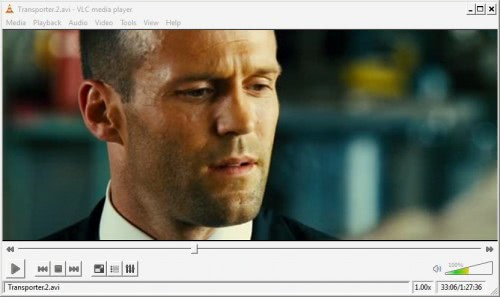
\includegraphics[height=5cm]{images/vlc1stVersion}
\par\end{centering}
\caption{Captura de la primera versió de VLC\label{fig:VLC1}}
\end{figure}

LibVLC no està tant pensat per utilitzar-lo desde terminal com podria
ser FFmpeg, i encara que també es pot integrar a qualsevol projecte,
és més complicat de instalar i utilitzar \cite{libVLCSampleCode}.\\

\lstinputlisting[breaklines=true,captionpos=b,frame=tb,language=C,caption={Codi base d'exemple de libVLC},label={libVLCSample}]{code/vlcExemple.txt}

\section{Proposició}

\subsection{Comparació: Ventatges i desventatges de cada eina}

Està clar que cada eina té les seves ventatges i desventatges, tampoc
hi ha una que sigui millor que l'altre, sinó que depèn del projecte
que es vulgui fer les solucions seran molt diferents. A continuació
s'analitzaran els pros i contres de cada eina, desde un punt de vista
subjectiu pel projecte que es vol fer:

\begin{table}[H]
\begin{tabular}{|>{\centering}m{2.5cm}|>{\centering}m{2.5cm}|>{\centering}m{2.5cm}|>{\centering}m{2.5cm}|}
\cline{2-4} \cline{3-4} \cline{4-4} 
\multicolumn{1}{>{\centering}m{2.5cm}|}{} & \textbf{Chrome Headless} & \textbf{Unreal Engine 4} & \textbf{Unity}\tabularnewline
\hline 
\textbf{Pros} & Simplicitat, alta compatibilitat, no requereix utilitzar plugins & És professional, millor qualitat d'iluminació & Molta documentació, molts plugins open-source, optimitzat per escenes
senzilles, alta compatibilitat\tabularnewline
\hline 
\textbf{Contres} & Pot quedar limitat en quant a potència; efectes de video & Relativament poca documentació, no tants plugins i comunitat com la
competència, poca compatibilitat amb Linux & Menys potent que Unreal, eines externes no professionals creades per
la comunitat\tabularnewline
\hline 
\end{tabular}

\caption{Comparativa subjectiva de les possibles eines}
\end{table}

\subsection{Elecció de l'eina i justificació}

Per poder decidir amb criteri i assegurar-se de que es prèn la decisió
correcte sobre quina és l'eina que s'ha de utilitzar, es farà una
prova amb cada una de les eines esmentades (Chrome Headless, Unreal
Engine 4 i Unity).\\

\subsubsection{Chrome Headless}

És molt útil per tasques automatitzades, no es necessita cap tipus
de software extra, com a molt es poden necessitar llibreries de nodejs
pels scripts de javascripts, però en tot cas, quedaria tot empaquetat
en un sol projecte. Al utilitzar el navegador de Chrome, això ens
dona moltes ventatges en quant a simplicitat de les tasques, però
també ens limita la potència, compatibilitat de códecs i formats,
pel que mai serà exactament igual que si executéssim les mateixes
tasques de manera nativa al ordinador.\\

Si busquem projectes creats amb aquesta eina que s'assemblin a l'objectiu
que volem aconseguir, trobem una aplicació creada per <<Sebastian
Pereyro>>, de la web Empirical \cite{HeadlessChromeProject}. Headless
Chrome està disponible a partir de la versió 59, acutalment van per
la 91, pel que no seria cap problema utilitzar aquesta eina. Es poden
carregar pàgines web i executar tests o tasques, a més de generar
PDFs i fer captures de pantalla repetidament. A més comenta que es
pot compartir de manera directa el contingut <<Screencast content>>,
això si, fent múltiples captures de pantalla. L'experiment que es
va proposar va ser de capturar àudio i video de manera automàtica,
tant d'una web pròpia com d'una web externa i transmetre el contingut
a Facebook, Youtube, Twitch...

El que utilitza com a eines, són Node.js, el navegador Headless Chrome
en qüestió, Pulseaudio que és el motor de video que utilitzarà per
la captura, i FFmpeg que farà la transmisió final del flux de Headless
Chrome cap a les destinacions pertinents. Tot això ho vol fer utilitzant
un servidor que s'ocupi de totes les tasques. Tenint una aplicació
client, en aquest cas farà ús de Postman \cite{Postman}, es comunica
amb el servidor central que tindrà tota la programació, agafa el contingut
multimèdia d'un altre web, i l'envia als servidors multimedia.

\begin{figure}[H]
\begin{centering}
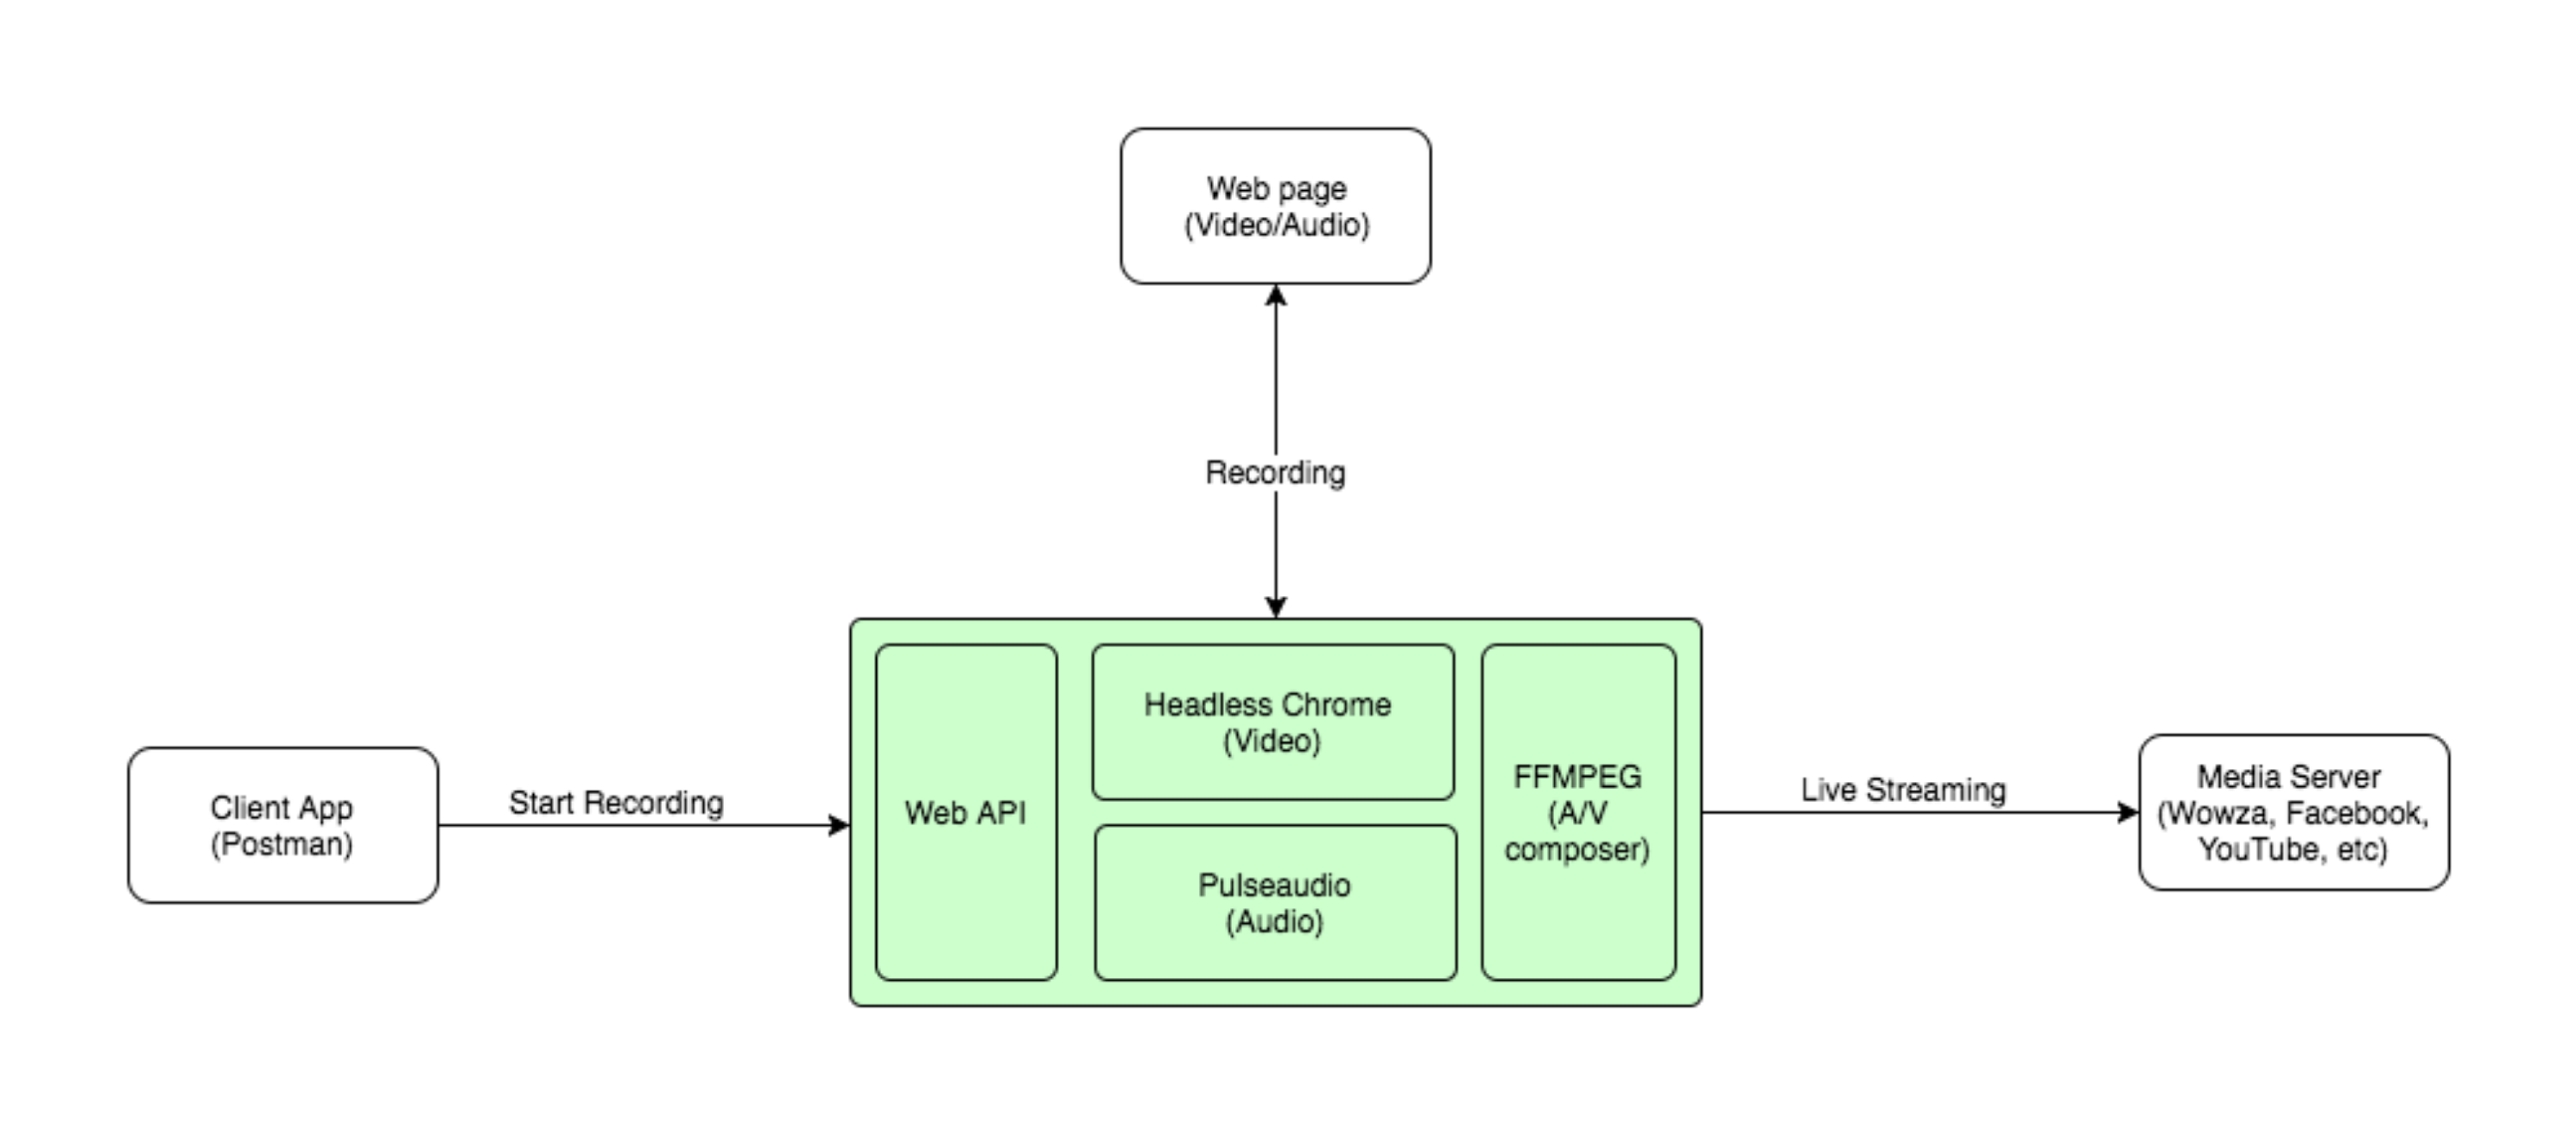
\includegraphics[height=5cm]{images/GraphHeadlessChromeEmpirical}
\par\end{centering}
\caption{Gràfic Experiment Headless Chrome\label{fig:ExperimentHCEmpirical}}
\end{figure}

\lstinputlisting[breaklines=true,captionpos=b,frame=tb,language=Java,caption={Experiment Headless Chrome Empirical},label={ExperimentEmpirical}]{code/ExperimentHCEmpirical.txt}

En el codi que ens proporciona \ref{ExperimentEmpirical}, podem comprovar
com fa la captura de la pantalla. Es tracta de una captura total de
la finestra del navegador. Per a fer-ho, utilitza una funció integrada
al Chrome, anomenada startScreencast. Pels paràmetres de configuració
que necessita i veient la documentació de Chrome DevTools \cite{ChromeDevTools},
podem deduir que es tracta un petit script que envia la comanda de
fer captura de pantalla, en el format que desitjem (en el cas d'exemple
és en jpeg), i junta aquests frames per aconseguir tenir un video.
En quant a l'àudio, ens comenta que encara que era un dels seus reptes,
no està suportat per Chrome, pel que no es podrà capturar de manera
nativa. La opció més vàlida serà capturar-lo per separat, i més tard
juntar-ho, el que farà que hi hagi problemes de sincronització d'àudio/video,
un problema molt comú en aquest tipus de projectes. La qualitat dels
videos tampoc podrà ser molt alta, ja que headless chrome no suporta
acceleració per hardware amb GPU, ho veiem a l'exemple \ref{chrome}
amb el flag --disable-gpu extret directament de la documentació de
Google \cite{HeadlessChromeDevel}. Un altre cosa que comenta és que
el framerate serà variable, nosaltres podem enviar 30 comandes per
segon de que faci la captura de pantalla, però és pràcticament impossible
que vagi totalment sincronitzat i faci exactament les 30 captures
cada segon, un dels problemes que comporta això, és que s'anirà desincronitzant
poc a poc, cada cop més, l'àudio.

Després de fer totes les captures, o mentres s'estan fent, es pot
utilitzar FFmpeg per juntar les imatges en una seqüència de video,
juntar-li l'àudio, i transmetre-ho a on es desitji, ja sigui en directe
o a un fitxer local.

En aquest projecte, no s'ha utilitzat cap eina d'automatització de
navegador, sinó que s'ha fet tot amb Headless Chrome Vanilla. Pel
que es farà una prova utilitzant totes les eines del projecte, i a
més, amb Puppeteer per poder-ho automatitzar tot.

Per la primera prova, es programarà tot en HTML i Javascript. Per
una banda tindrem el index.html, un arxiu molt senzillet que contindrà
un o dos videos locals que es reproduiràn automàticament a dins un
canvas, al obrir l'arxiu.\\

\lstinputlisting[breaklines=true,captionpos=b,frame=tb,language=HTML,caption={Test Chrome Headless | index.html},label={TestCHindex}]{code/tests/headlessChrome/index.html}

L'aspecte de la web és correcte, tenim un video, concretament, el
tràiler de la película Nightcrawler \cite{Nightcrawler} ocupant tota
la pantalla en el fons, i a la cantonada superior esquerra, ocupant
un quart de la pantalla tenim el tràiler de la película Stalker \cite{Stalker}.

\begin{figure}[H]
\begin{centering}
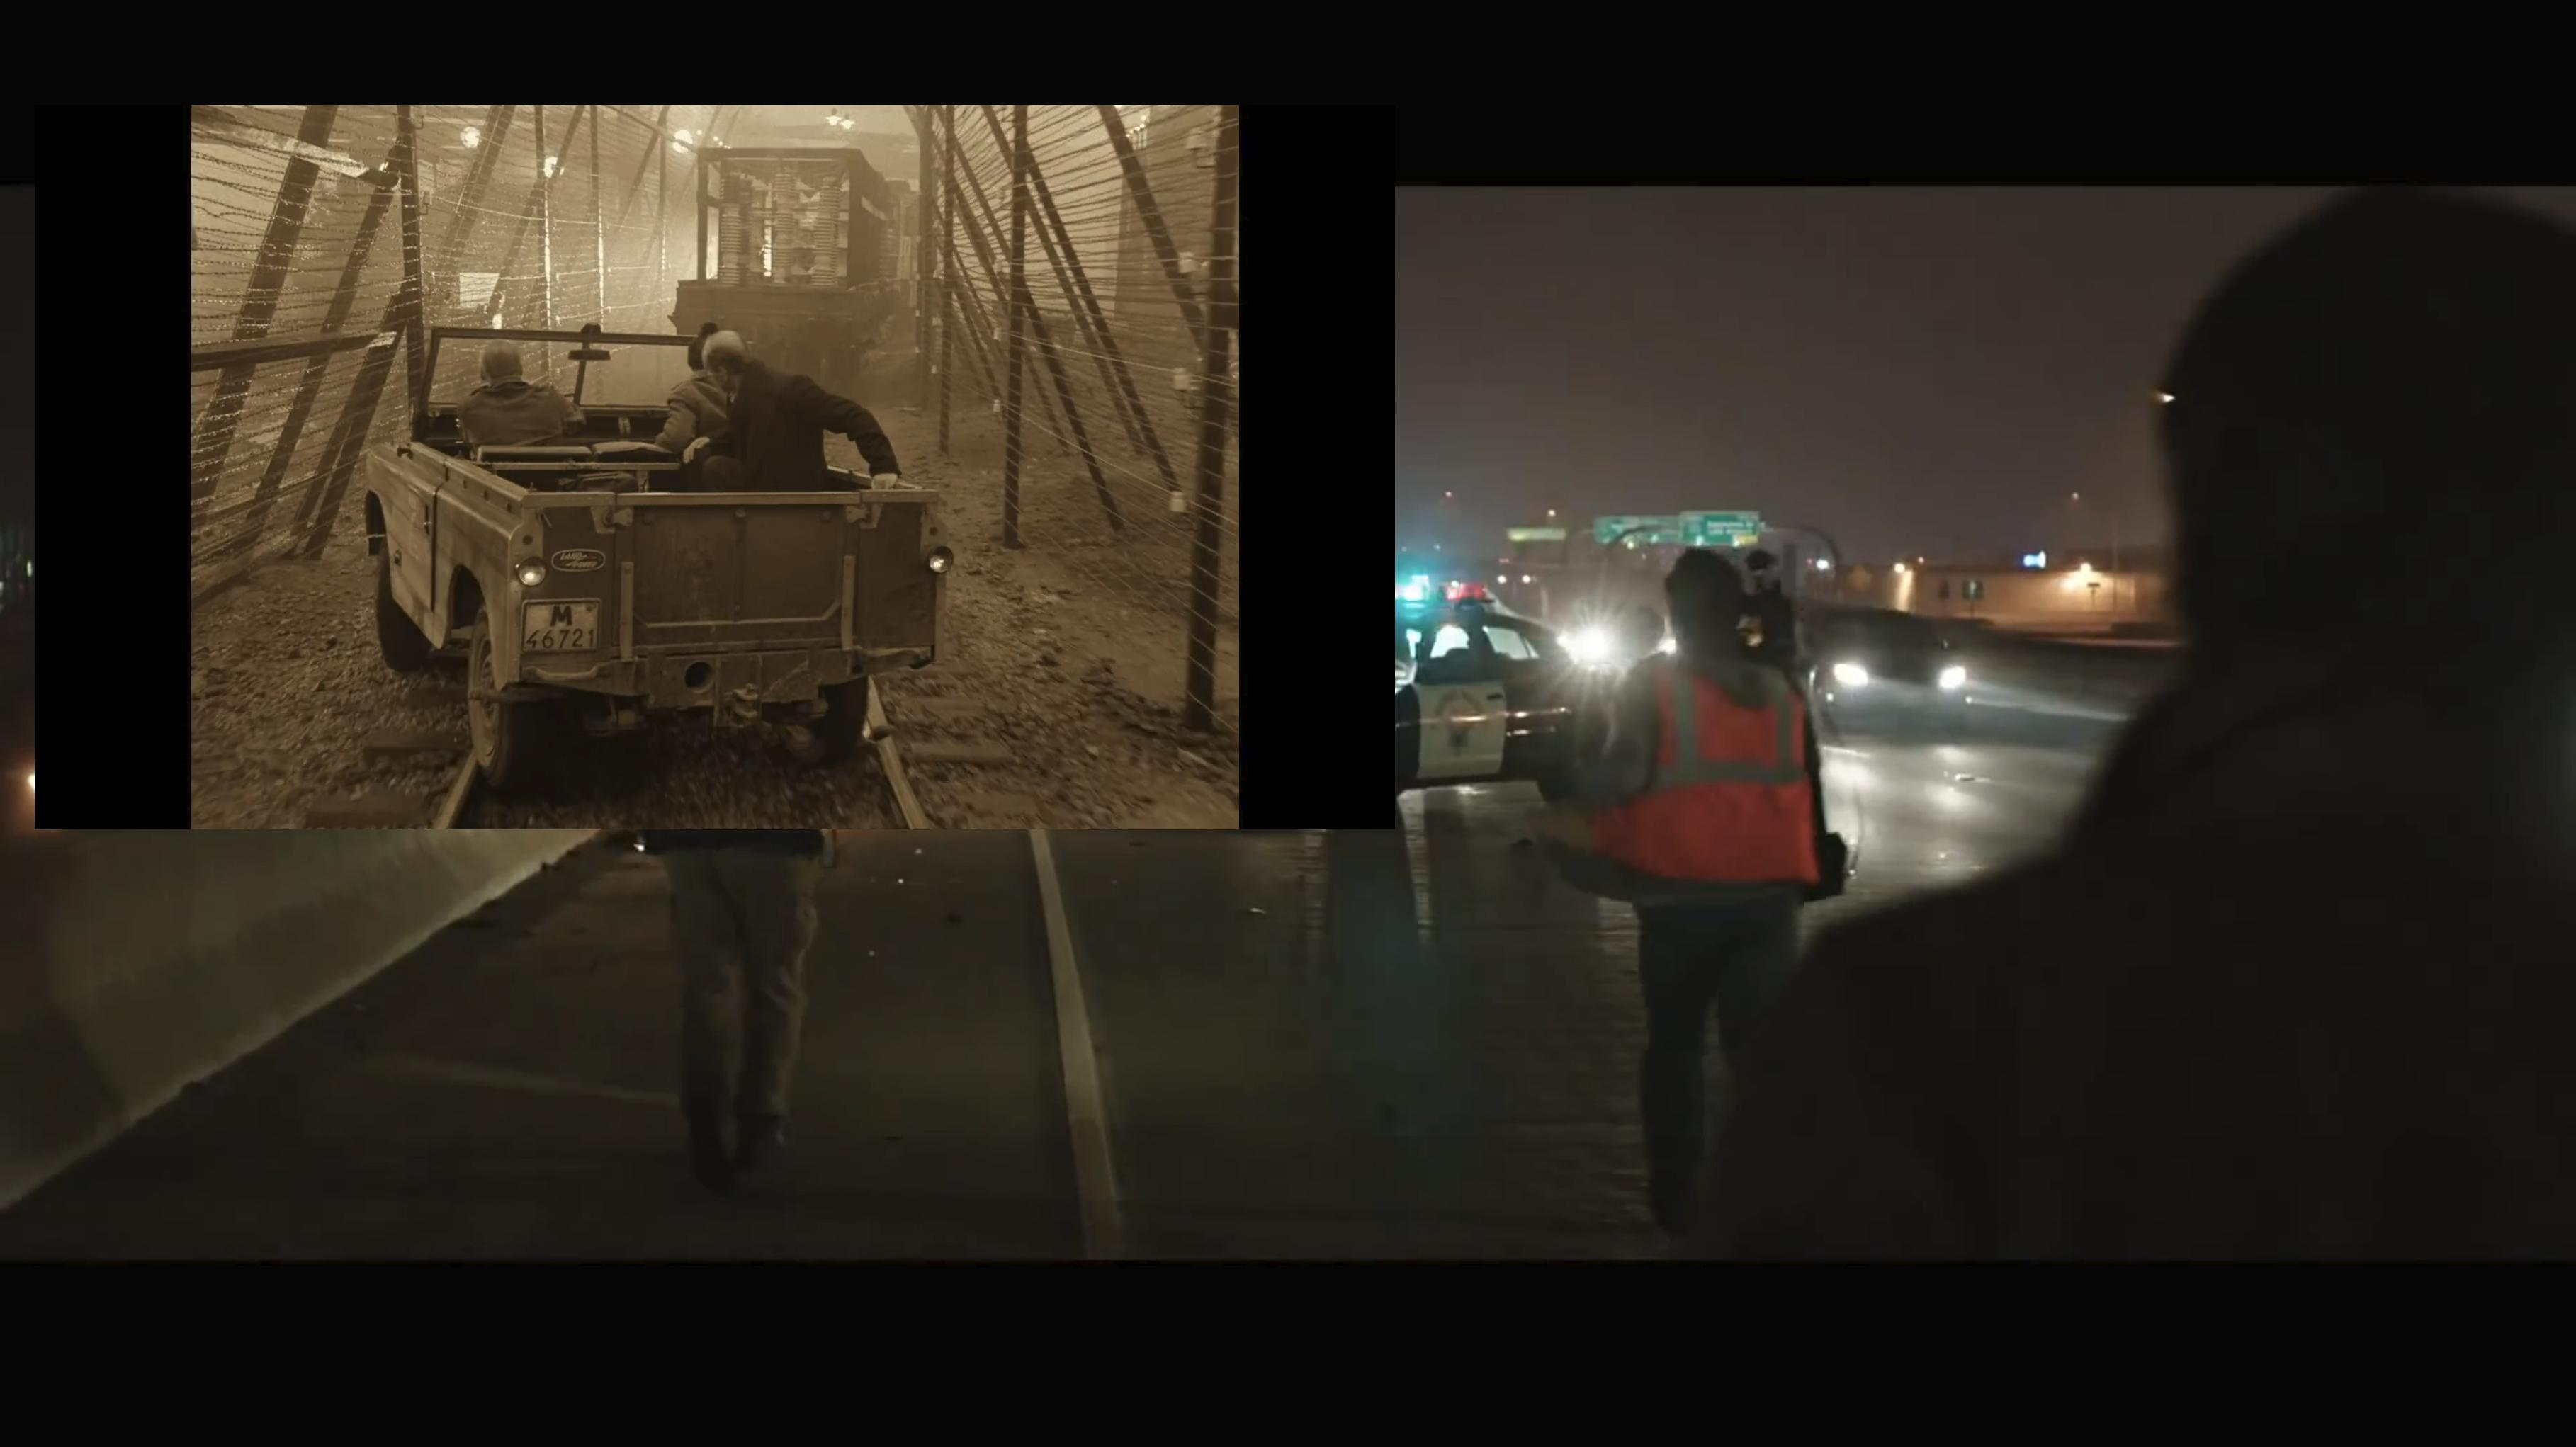
\includegraphics[height=6cm]{images/tests/CHindexhtml}
\par\end{centering}
\caption{Resultat index.html\label{fig:HCTestindexhtml}}
\end{figure}

Un dels primers problemes que han sorgit, ha sigut amb la reproducció
dels videos, degut a que un navegador no està pensat exclusivament
per aquestes funcions, les seves polítiques d'ús poden canviar dràsticament
d'un dia per l'altre i destrossar un projecte d'aquest estil. Tant
és així que a l'any 2017, van introduir una nova política a la versió
71, en la que no estava permès auto reproduir els videos automàticament
al obrir una web, sinó que el usuari havia de clicar manualment al
video. Això si, permetia reproduir-los si estaven sense so. Una política
probablement introduida per evitar el ús de publicitat molesta, però
que hauria canviat per complet aquest projecte i hauria fet que deixés
de funcionar. Per tant, les opcions que es tenen, és reproduir els
videos sense àudio (inviable ja que l'àudio és un dels requisits),
o utilitzar una eina externa com Puppeteer per fer <<trampes>> i
clicar allà on volguem fent creure al navegador que ho està fent un
usuari qualsevol.\\

\lstinputlisting[breaklines=true,captionpos=b,frame=tb,language=Java,caption={Test Reproducció Videos | videoPlayback.js},label={TestCHvideoPlayback}]{code/tests/headlessChrome/videoPlayback.js}

Amb aquest codi ja tindrem uns scripts que guardaran 30 captures per
segon a una carpeta local. A la vegada, podem executar una comanda
FFmpeg, per convertir aquestes captures en una seqüència de video,
i guardar-ho a un arxiu local. Això ho podrem aconseguir amb aquesta
sèrie de comandes a la terminal.\\

\lstinputlisting[breaklines=true,captionpos=b,frame=tb,language=bash,caption={Comandes FFmpeg},label={TestCHffmpeg}]{code/tests/headlessChrome/ffmpegCommands.txt}

Pel FFmpeg s'utilitzen els flags:
\begin{itemize}
\item -r 24: indica el número de frames per segon que tindra el video resultant.
\item -pattern\_type glob \cite{FFmpegPatternType}: indiquem el patró del
nom dels arxius per una lectura correcte, en aquest cas ens ajudavem
d'un txt que contenia tots els noms dels arxius, generat automàticament
pel javascript.
\item -re: indica que el processament s'ha de fer amb una velocitat de 1x,
per evitar que processi les imatges més ràpid de 24 FPS i es vegi
més ràpid del que hauria.
\end{itemize}
%
Aquesta solució no ha donat uns resultats gaire atractius, sobretot
pel fet d'estar capturant la pantalla amb screenshots, i sense poder
transmetre el àudio. Pel que s'ha provat un altre alternativa, basada
en un altre projecte creat per l'usuari de Github FBSamples \cite{FBSamplesRepo}.

En aquesta altre proposta, trobem algunes variants interessants, el
més diferent és que utilitza un servidor de websockets com a intermediari. 

\begin{figure}[H]
\begin{centering}
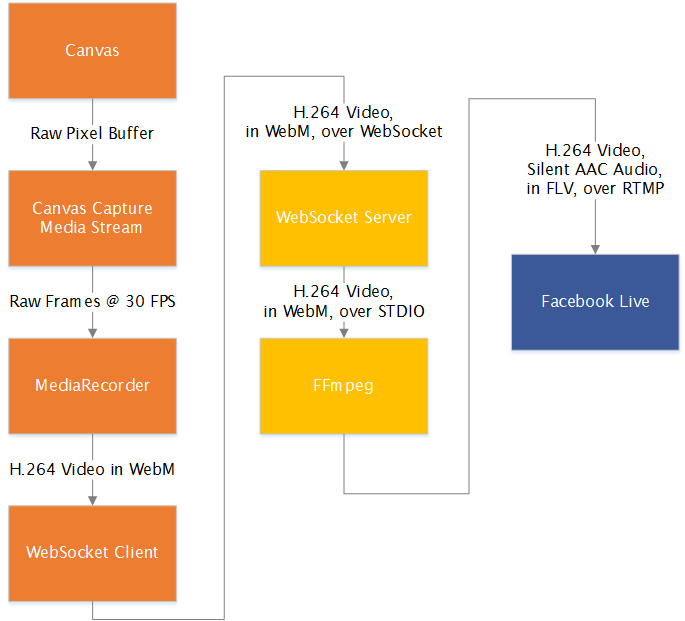
\includegraphics[height=8cm]{images/tests/architectureFacebookCanvas}
\par\end{centering}
\caption{Arquitectura Projecte Canvas Streaming\label{fig:HCCanvasStreaming}}
\end{figure}

Això sí, per capturar el canvas, utilitza MediaRecorder, que és el
mateix plugin que s'utilitzava en la primera prova. Fent algunes modificacions
al projecte de github de prova obtenim resultats amb el html creat
anteriorment.\\

\lstinputlisting[breaklines=true,captionpos=b,frame=tb,language=Java,caption={Servidor Websockets | server.js},label={TestCHserver}]{code/tests/headlessChrome/server.js}

Les ventatges amb aquest canvi és que aconseguim molta més qualitat
de imatge, i es captura automàticament el so. Per altre banda, es
segueix utilitzant Pulseaudio de manera autònoma, pel que seguirà
havent un retard variant de video/àudio.

Les conclusions que es treuen d'aquest experiment és que aquesta eina
és interessant per fer algun petit projecte o que no requereixi de
so, però no acaba d'encaixar en els requisits que es proposaven.\\

\subsubsection{Unreal Engine 4}

Per la prova amb Unreal Engine, s'ha utilitzat una tecnologia molt
utilitzada de manera professional a la televisió, i que recentment
ha estat integrada a Unreal com a plugin extern. Es tracta del software
NDI (Network Device Interface) \cite{NewTekNDI}. Creat per la empresa
NewTek i amb una llicència privativa, permet una gran qualitat d'imatge,
amb poc retard i una estructura molt estable. Dóna un grau important
de professionalitat i compta amb un suport per part de NewTek i un
fòrum de comunitat. Les desventatges són, que al ser una empresa que
recolza el software privatiu i tancat, no té cap mena de suport per
Linux, només per Windows i MacOS. Sumant això a que la compatibilitat
d'Unreal Engine tampoc és extraordinària, és bastant inabastable aconseguir
bons resultats amb Unreal en una màquina Linux. Per tant, les proves
que es faràn seran desde una màquina Windows per comprovar la potència
d'aquesta tecnologia. \\

Per començar, crearem un streaming de NDI desde VLC, per poder comprovar
que funciona correctament tant entrada com sortida de fluxos. Un cop
instalem les Tools de NDI, el plugin de VLC per poder treballar amb
aquest software, s'instalarà automàticament. Només cal entrar a les
opcions de VLC i marcar com a motor de sortida <<NewTek NDI Video
Output>>.

\begin{figure}[H]
\begin{centering}
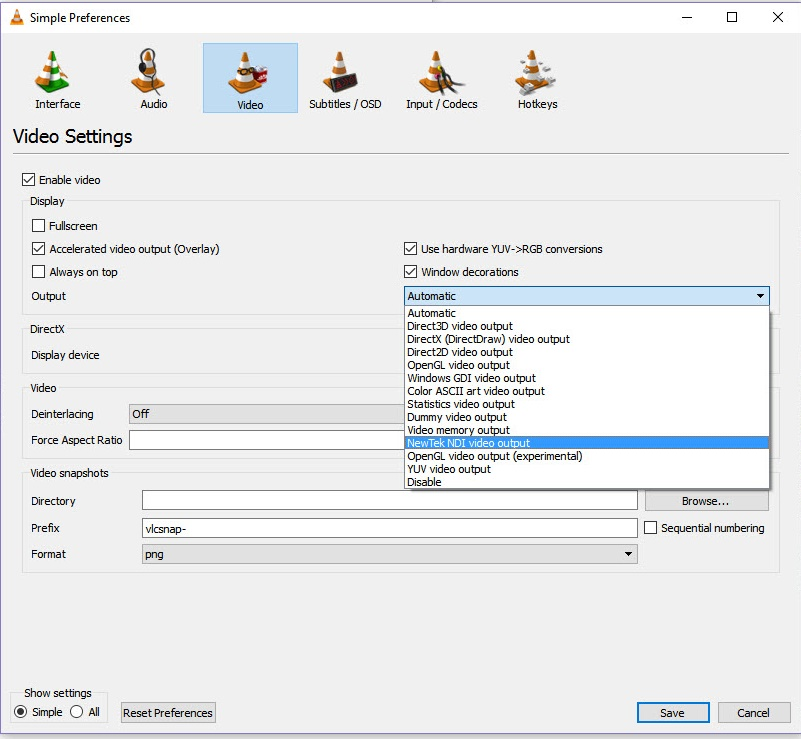
\includegraphics[height=9cm]{images/tests/NDIVLC}
\par\end{centering}
\caption{Configuració Sortida NDI a VLC\label{fig:NDIVLC}}
\end{figure}

Encara que per aquesta prova s'hagi fet la sortida amb VLC, es pot
fer de moltes altres maneres, com pot ser FFmpeg o una eina propia
de NDI dedicada a això.\\

Un cop ja tenim un flux de video creat, l'haurem de rebre a l'Unreal,
per fer-ho, hem d'utilitzar el plugin corresponent, i seguir els pasos
de la seva documentació \cite{NDI Unreal Documentation}.

\begin{figure}[H]
\begin{centering}
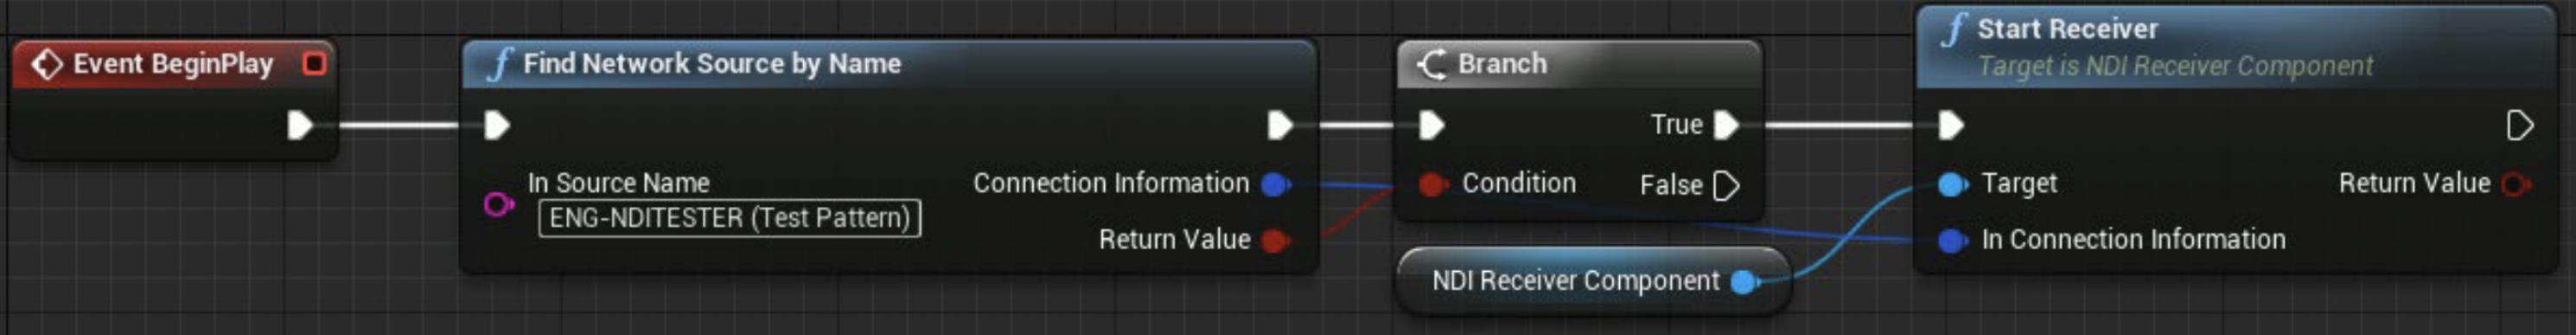
\includegraphics[height=1.5cm]{images/tests/NDIReceive.jpeg}
\par\end{centering}
\caption{Node NDI Receiver\label{fig:NDIReceiver}}
\end{figure}

Ara que ja està tot programat, ja comencem a veure alguns resultats
d'aquest software. Per aprofitar l'Unreal i provar altres efectes
també, s'ha escollit un video amb un chroma per comprovar com es comportava
devant un streaming calculant-lo a temps real.

\begin{figure}[H]
\begin{centering}
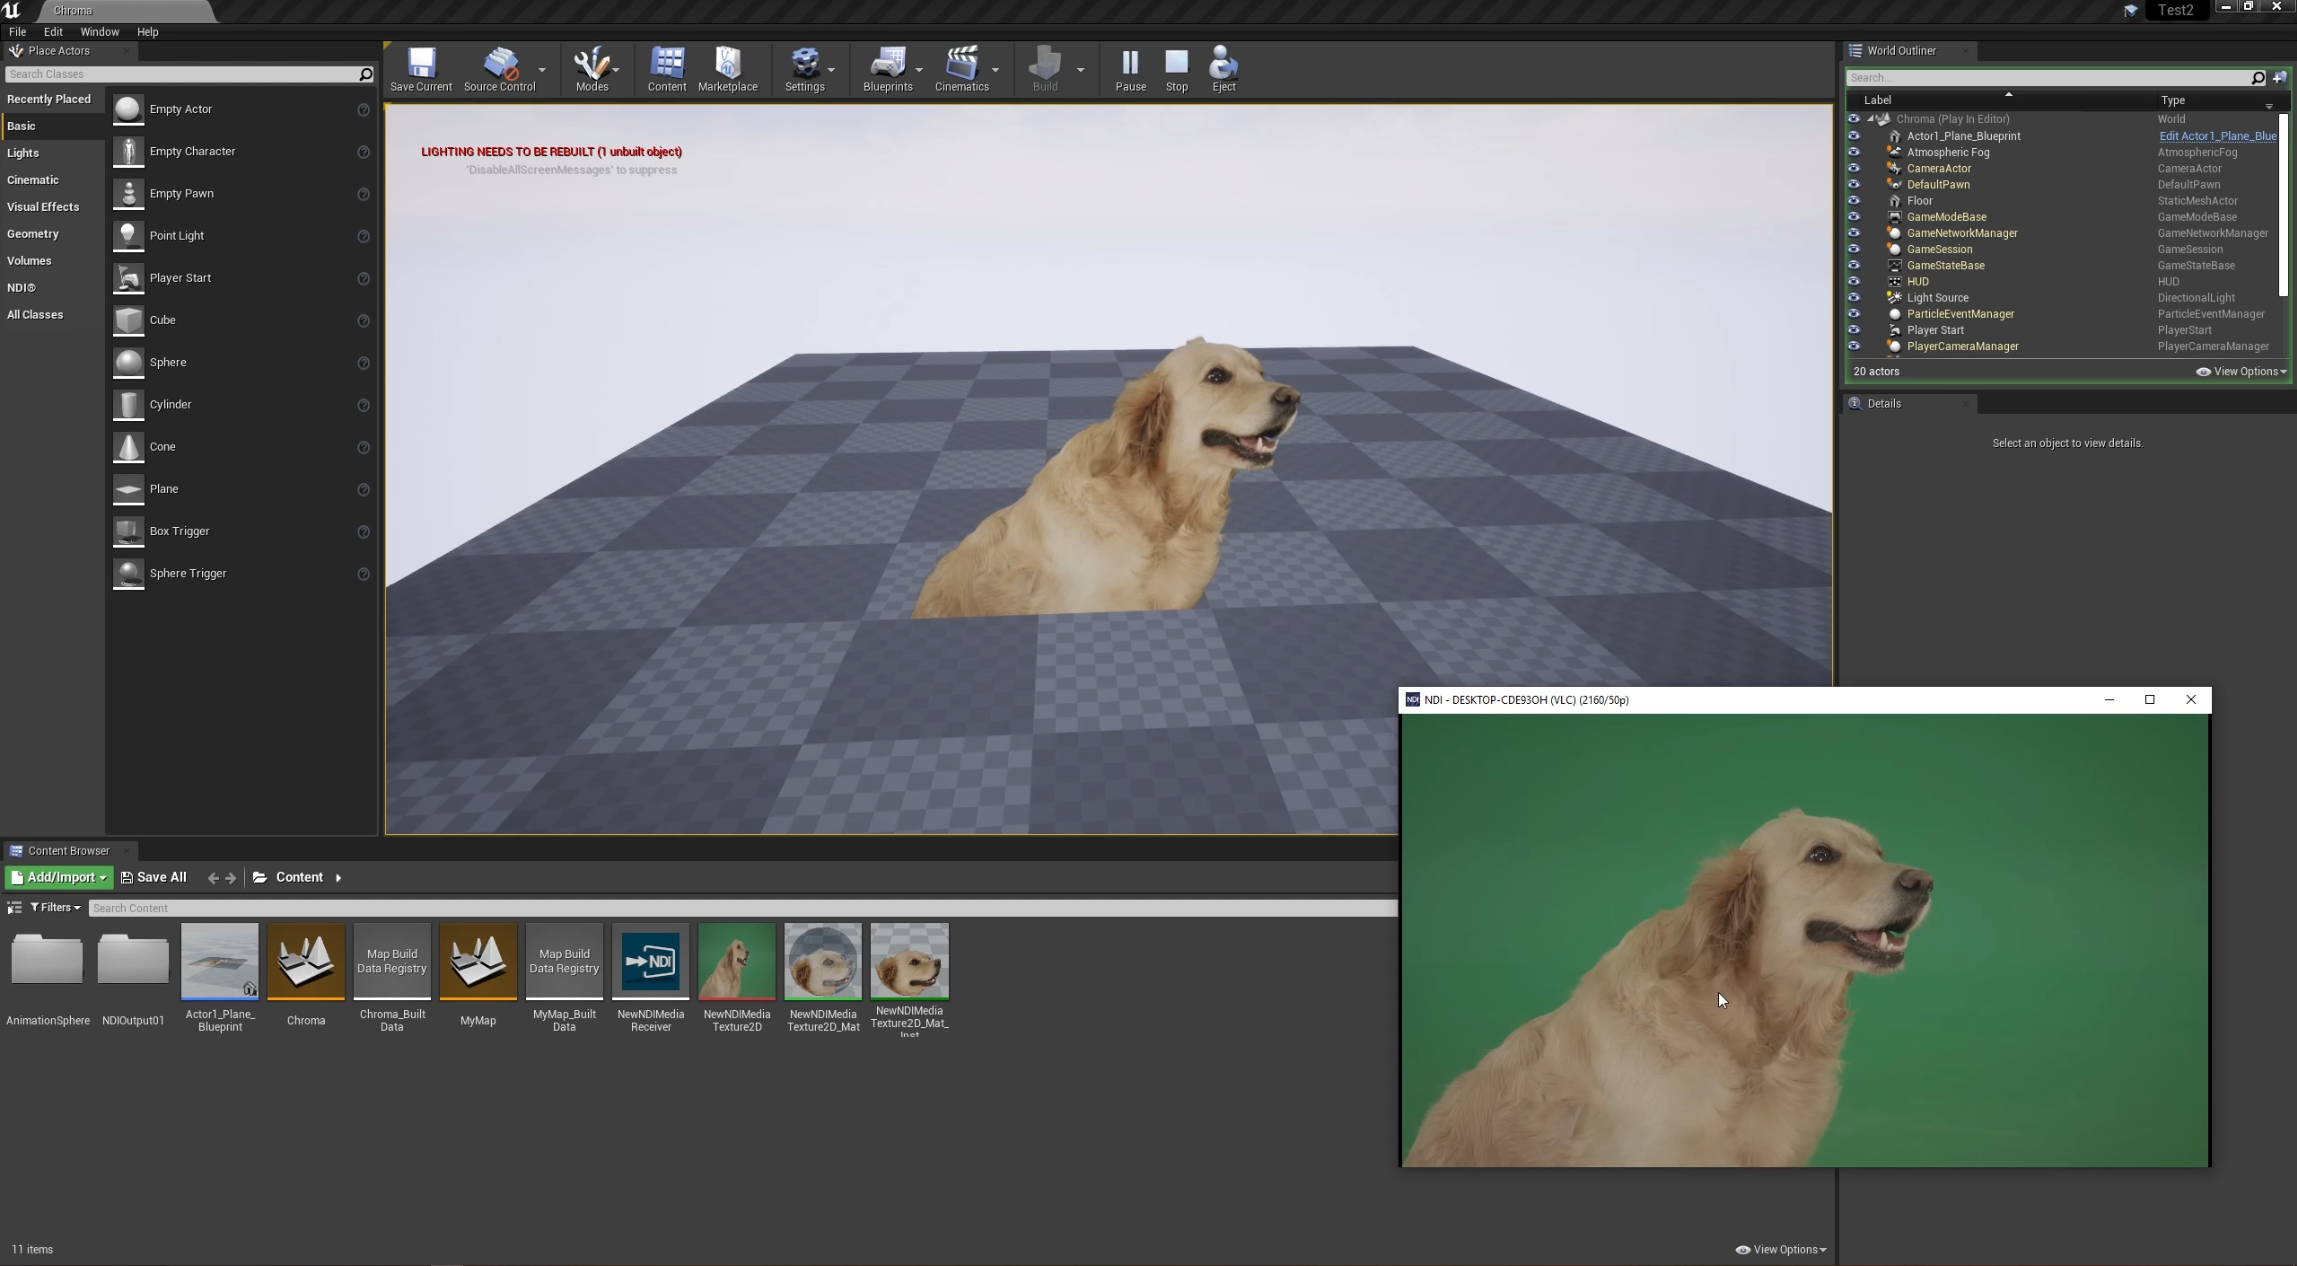
\includegraphics[height=7cm]{images/tests/UnrealNDI}
\par\end{centering}
\caption{Resultat NDI Input\label{fig:NDIReceiverResultat}}
\end{figure}

Els resultats d'aquesta prova han sigut molt bons, la latència del
NDI era molt baixa, a més d'una qualitat sorprenent. Ha donat alguns
problemes d'estabilitat en algun moment, però s'ha de tenir en compte
que el plugin d'Unreal encara és molt nou i és normal que doni algun
problema que altre, encara i això, són resultats prou estables i té
potencial per poder ser utilitzat com a eina de televisió professional.\\

\subsubsection{Unity}

Per la prova del Unity, s'ha creat un projecte que contigui diversos
elements. Un video de fons, un element 3D amb un video com a texture,
un logo 3D i un PNG amb transparència. Per a la reproducció de videos
s'ha escollit el plugin UMP (Universal Media Player) \cite{UMP Plugin},
considerat el reproductor més complert de tota l'Asset Store (plataforma
de descàrrega de plugins).

\begin{figure}[H]
\begin{centering}
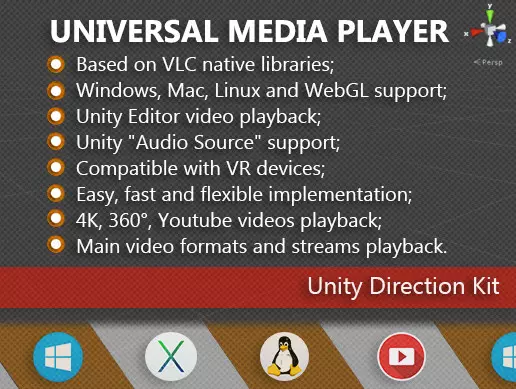
\includegraphics[height=7cm]{images/tests/UMPFunctions}
\par\end{centering}
\caption{Funcionalitats UMP\label{fig:UMPFunctions}}
\end{figure}

A més, és l'únic compatible amb Linux, el sistema operatiu més utilitzat
en sistemes al núvol \cite{Cloud Linux}. Pel UMP, haurem de posar
un element que controla la reproductor, i definir quines són les malles
que han de renderitzar el video. Per aquesta prova es té un controlador
que reproduirà el video del fons, i un altre que reproduirà el video
de la càpsula, l'altre element 3D. A més, tindrem una animació pel
logo 3D que anirà girant, i un altre per la capsula que s'anirà movent
per la pantalla.

\begin{figure}[H]
\begin{centering}
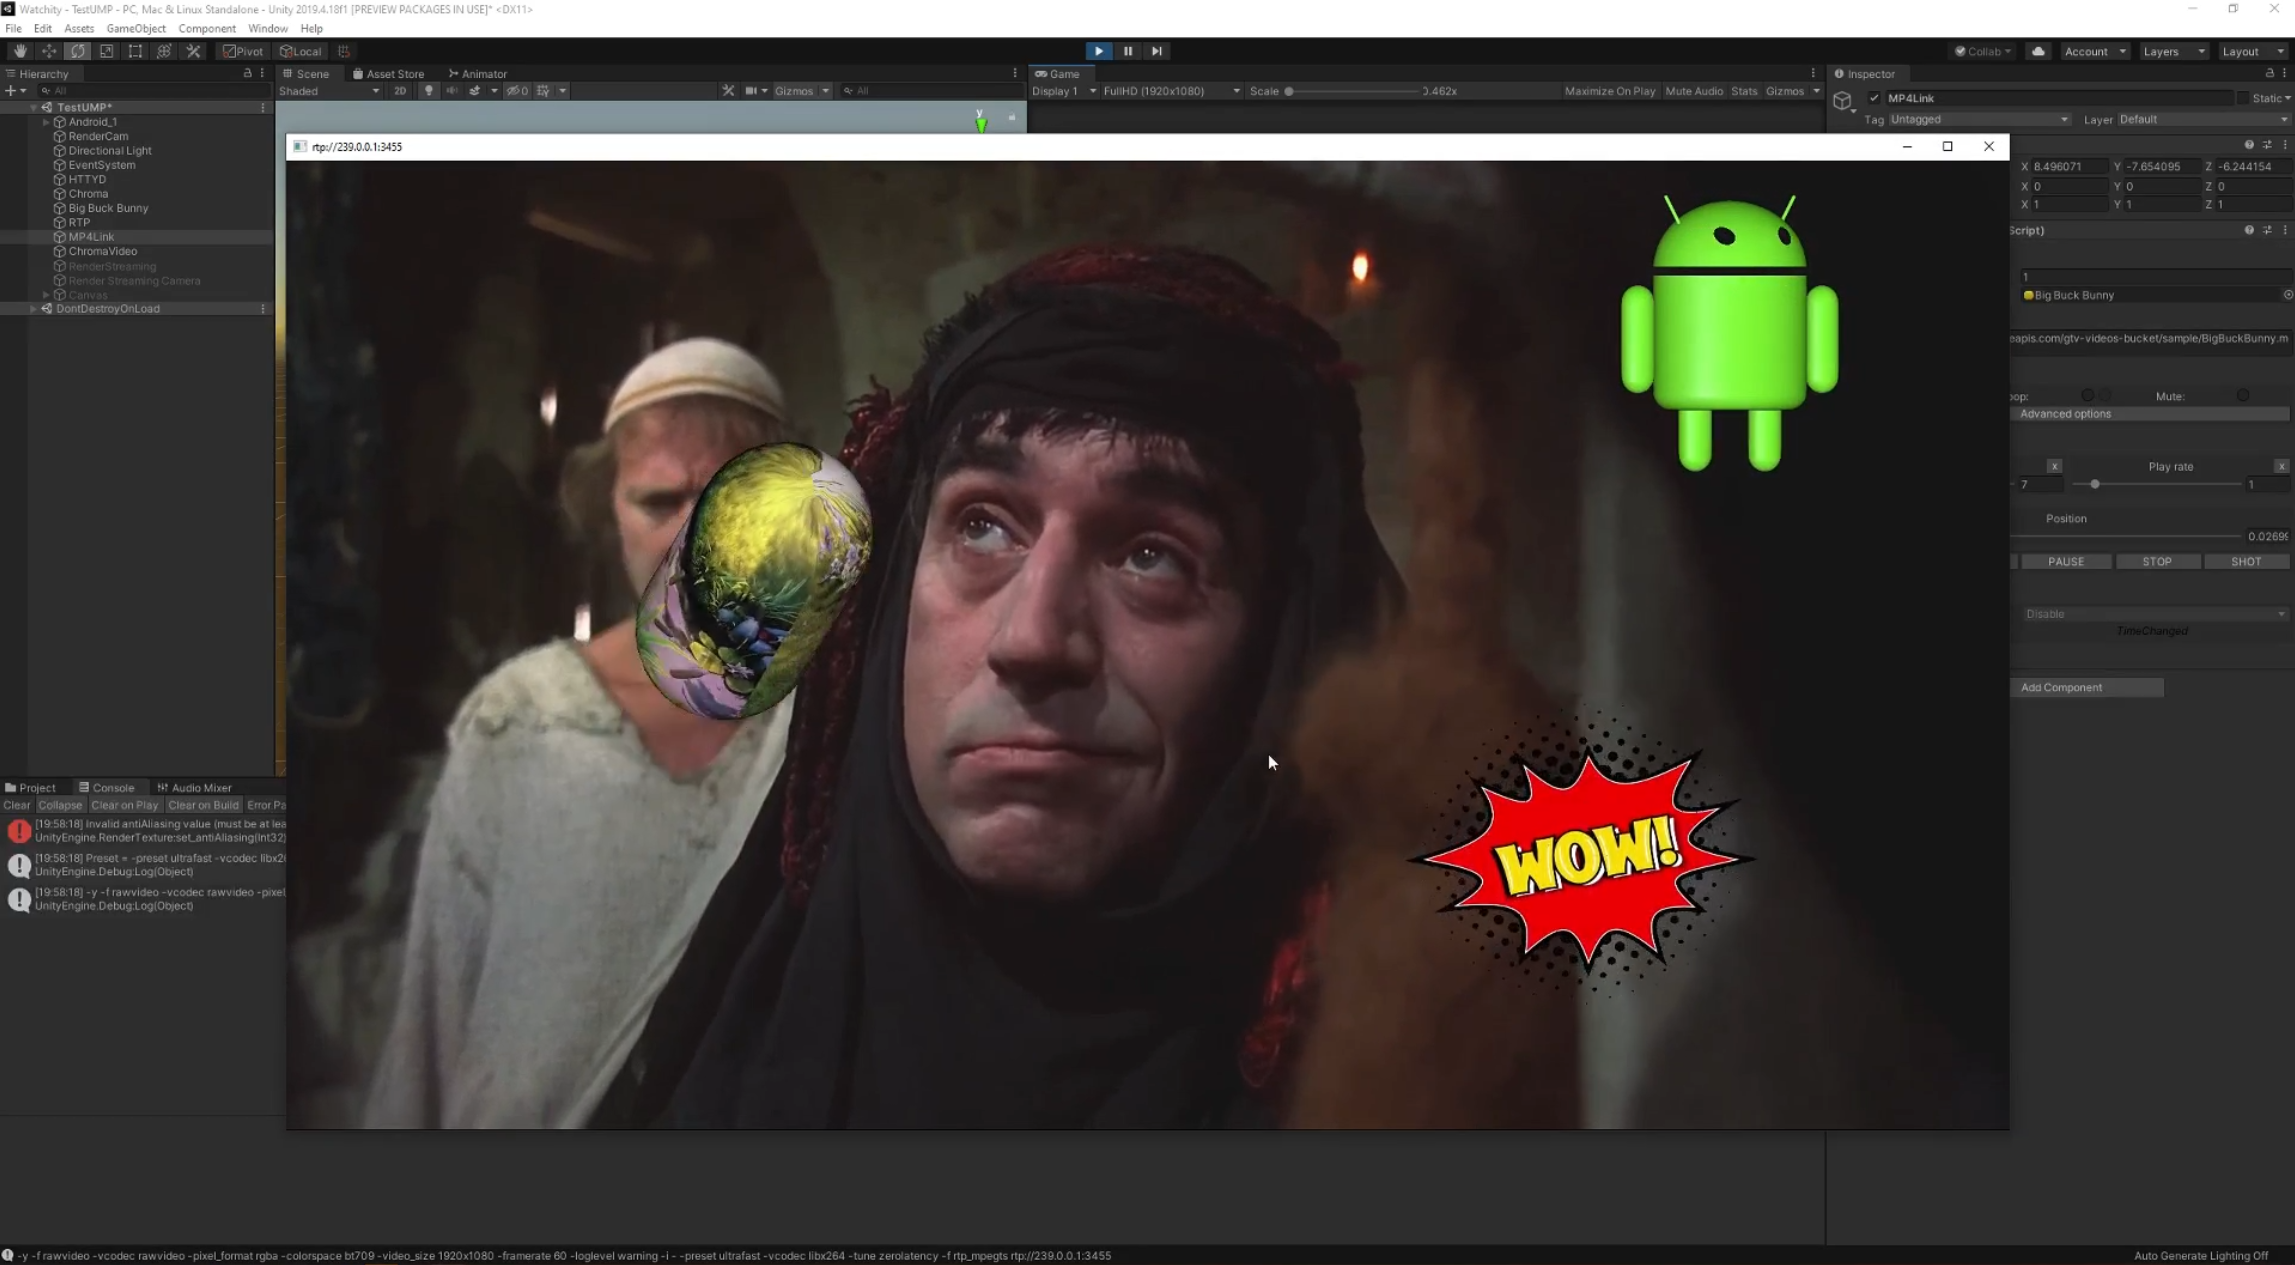
\includegraphics[height=7cm]{images/tests/UnityTest}
\par\end{centering}
\caption{Prova Unity\label{fig:ProvaUnity}}
\end{figure}

Els resultats amb Unity han sigut molt satisfactoris, no ha donat
cap problema i la reproducció ha sigut la més fluida. El plugin UMP
suporta pràcticament tot tipus de formats de videos ja que utilitza
les llibreries de libVLC. El codi és mitjanament obert pel que es
podrà editar fàcilment. La imatge en PNG té la transparència perfectament
aplicada, pel que veiem que el Unity suporta els valors d'alpha d'aquest.\\

Ara que ja s'han fet proves suficients amb totes les eines, es pot
decidir sense cap tipus de dubte, que la millor opció per aquest projecte
és \textbf{Unity}.\\

\subsection{Elecció de les llibreries a utilitzar}

\subsubsection{Entrada de fluxos}

Decidit Unity com a eina a utilitzar, el següent pas és escollir les
llibreries que permetran l'entrada de fluxos. Anteriorment s'han comentat
les dues més importants, que són FFmpeg i libVLC. A les proves del
Unity s'ha utilitzat un plugin anomenat UMP, el qual ha donat molts
bons resultats. S'ha decidit utilitzar-lo ja que fa ús de libVLC,
i ens ofereix una gran compatibilitat, a diferència d'altres com pot
ser AVPro \cite{AVPro}, molt més potent, però amb la desventatge
d'utilitzar llibreries pròpies i no ser compatible amb Linux.

Encara i apuntar tot a UMP, s'ha fet una prova comparativa dels dos
plugins, ambdós executant-se en el mateix sistema operatiu (Windows
10) i mateixes condicions, un video molt pesat en resolució 8K. 

\begin{figure}[H]
\begin{centering}
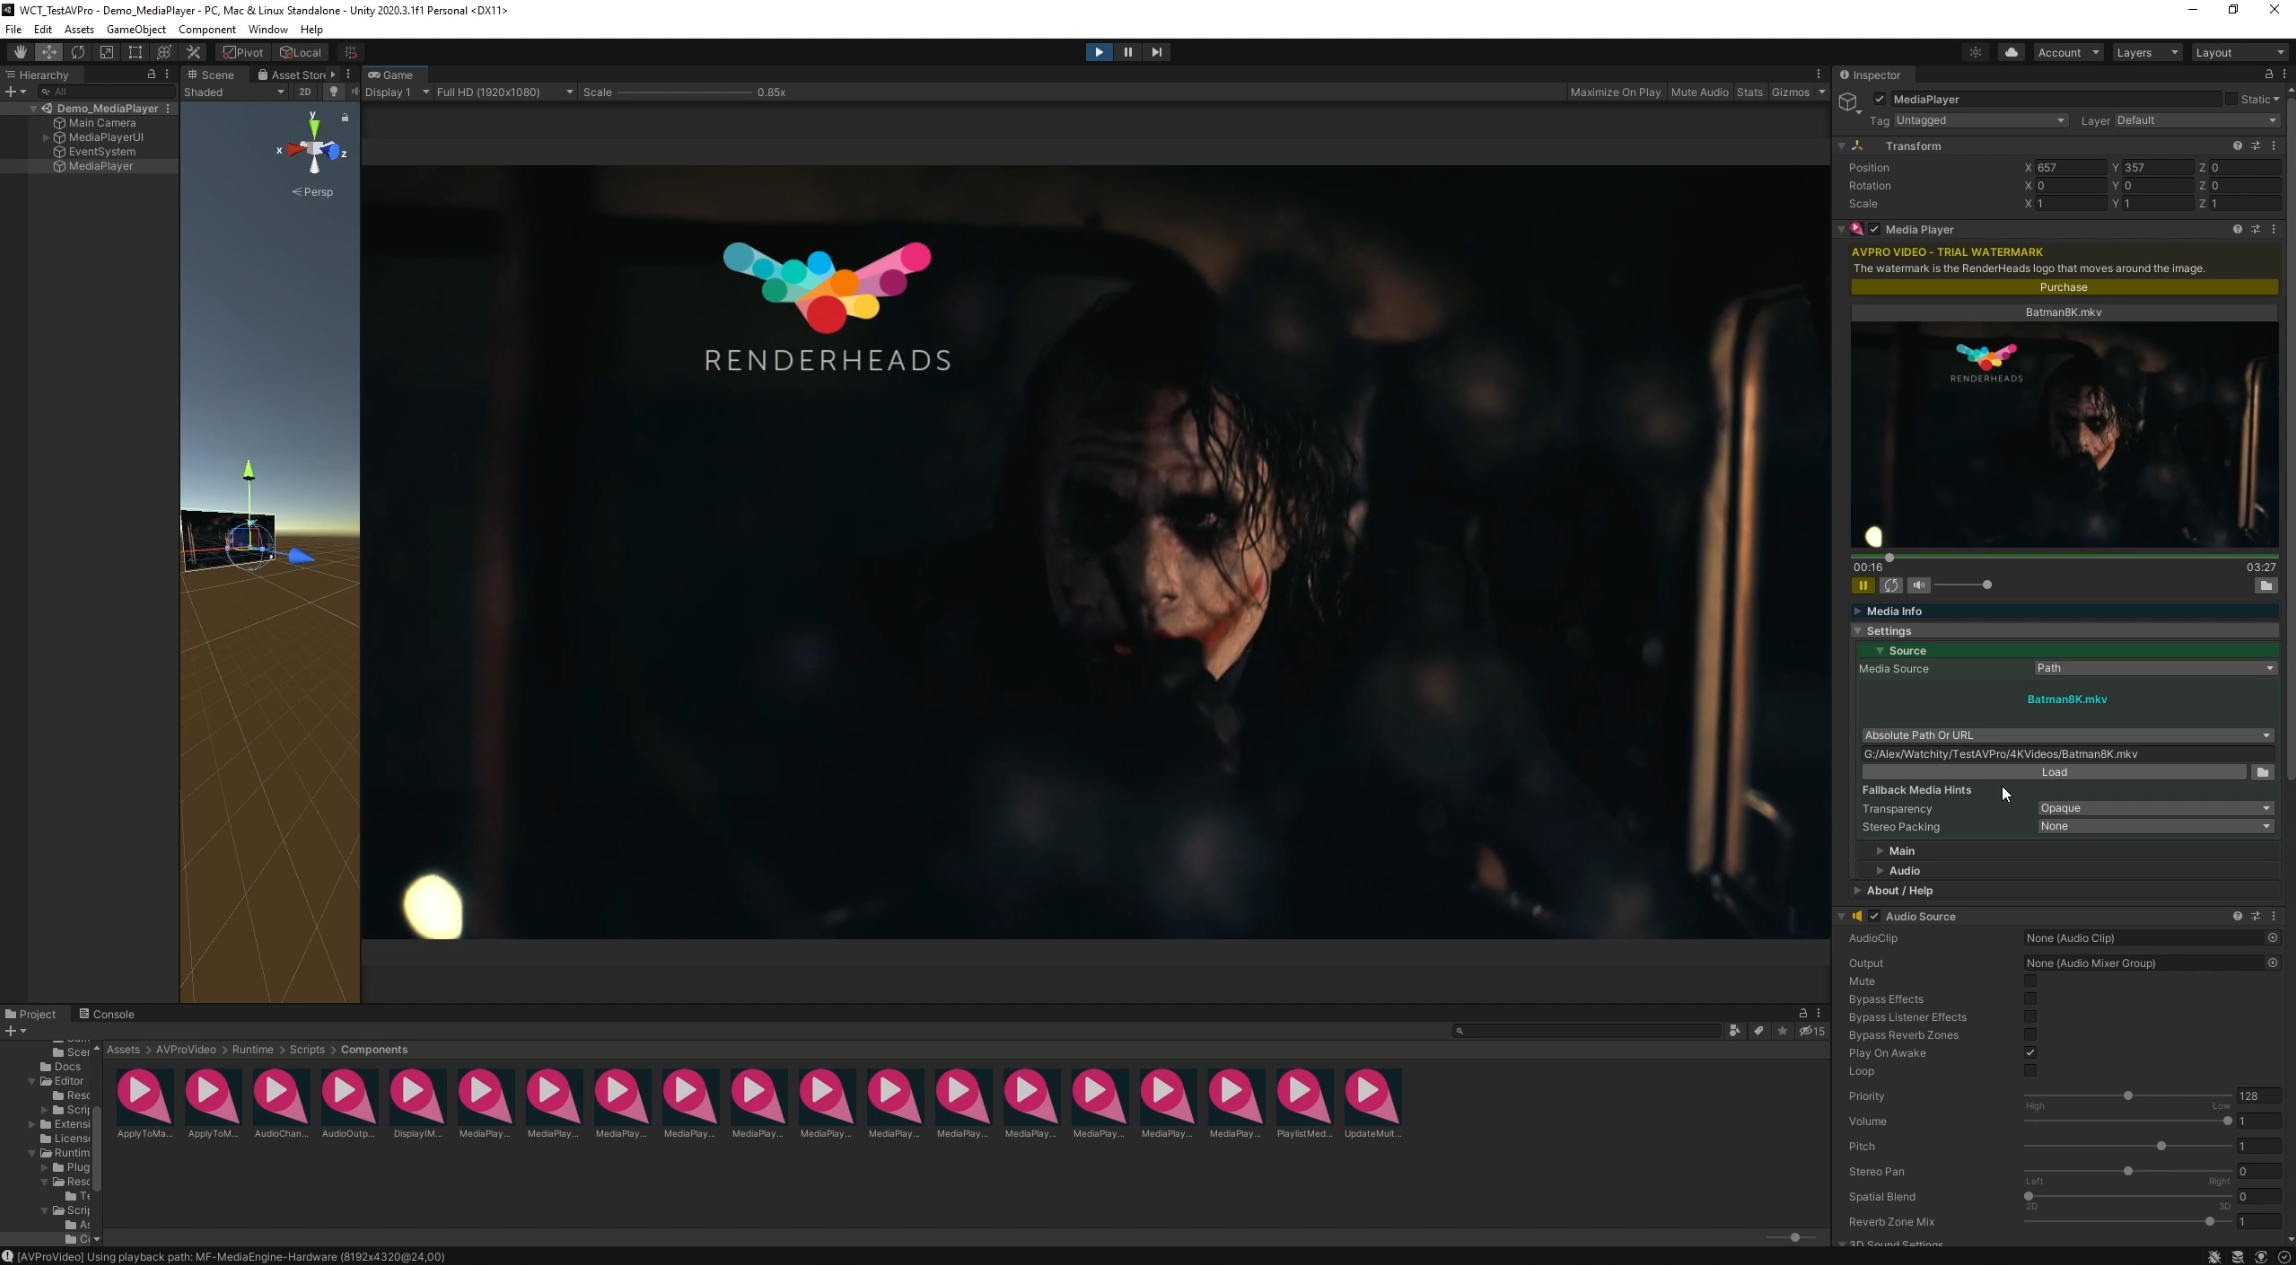
\includegraphics[height=7cm]{images/AVPro}
\par\end{centering}
\caption{Prova AVPro (Video 8K)\label{fig:AVProvsUMP}}
\end{figure}

\begin{figure}[H]
\begin{centering}
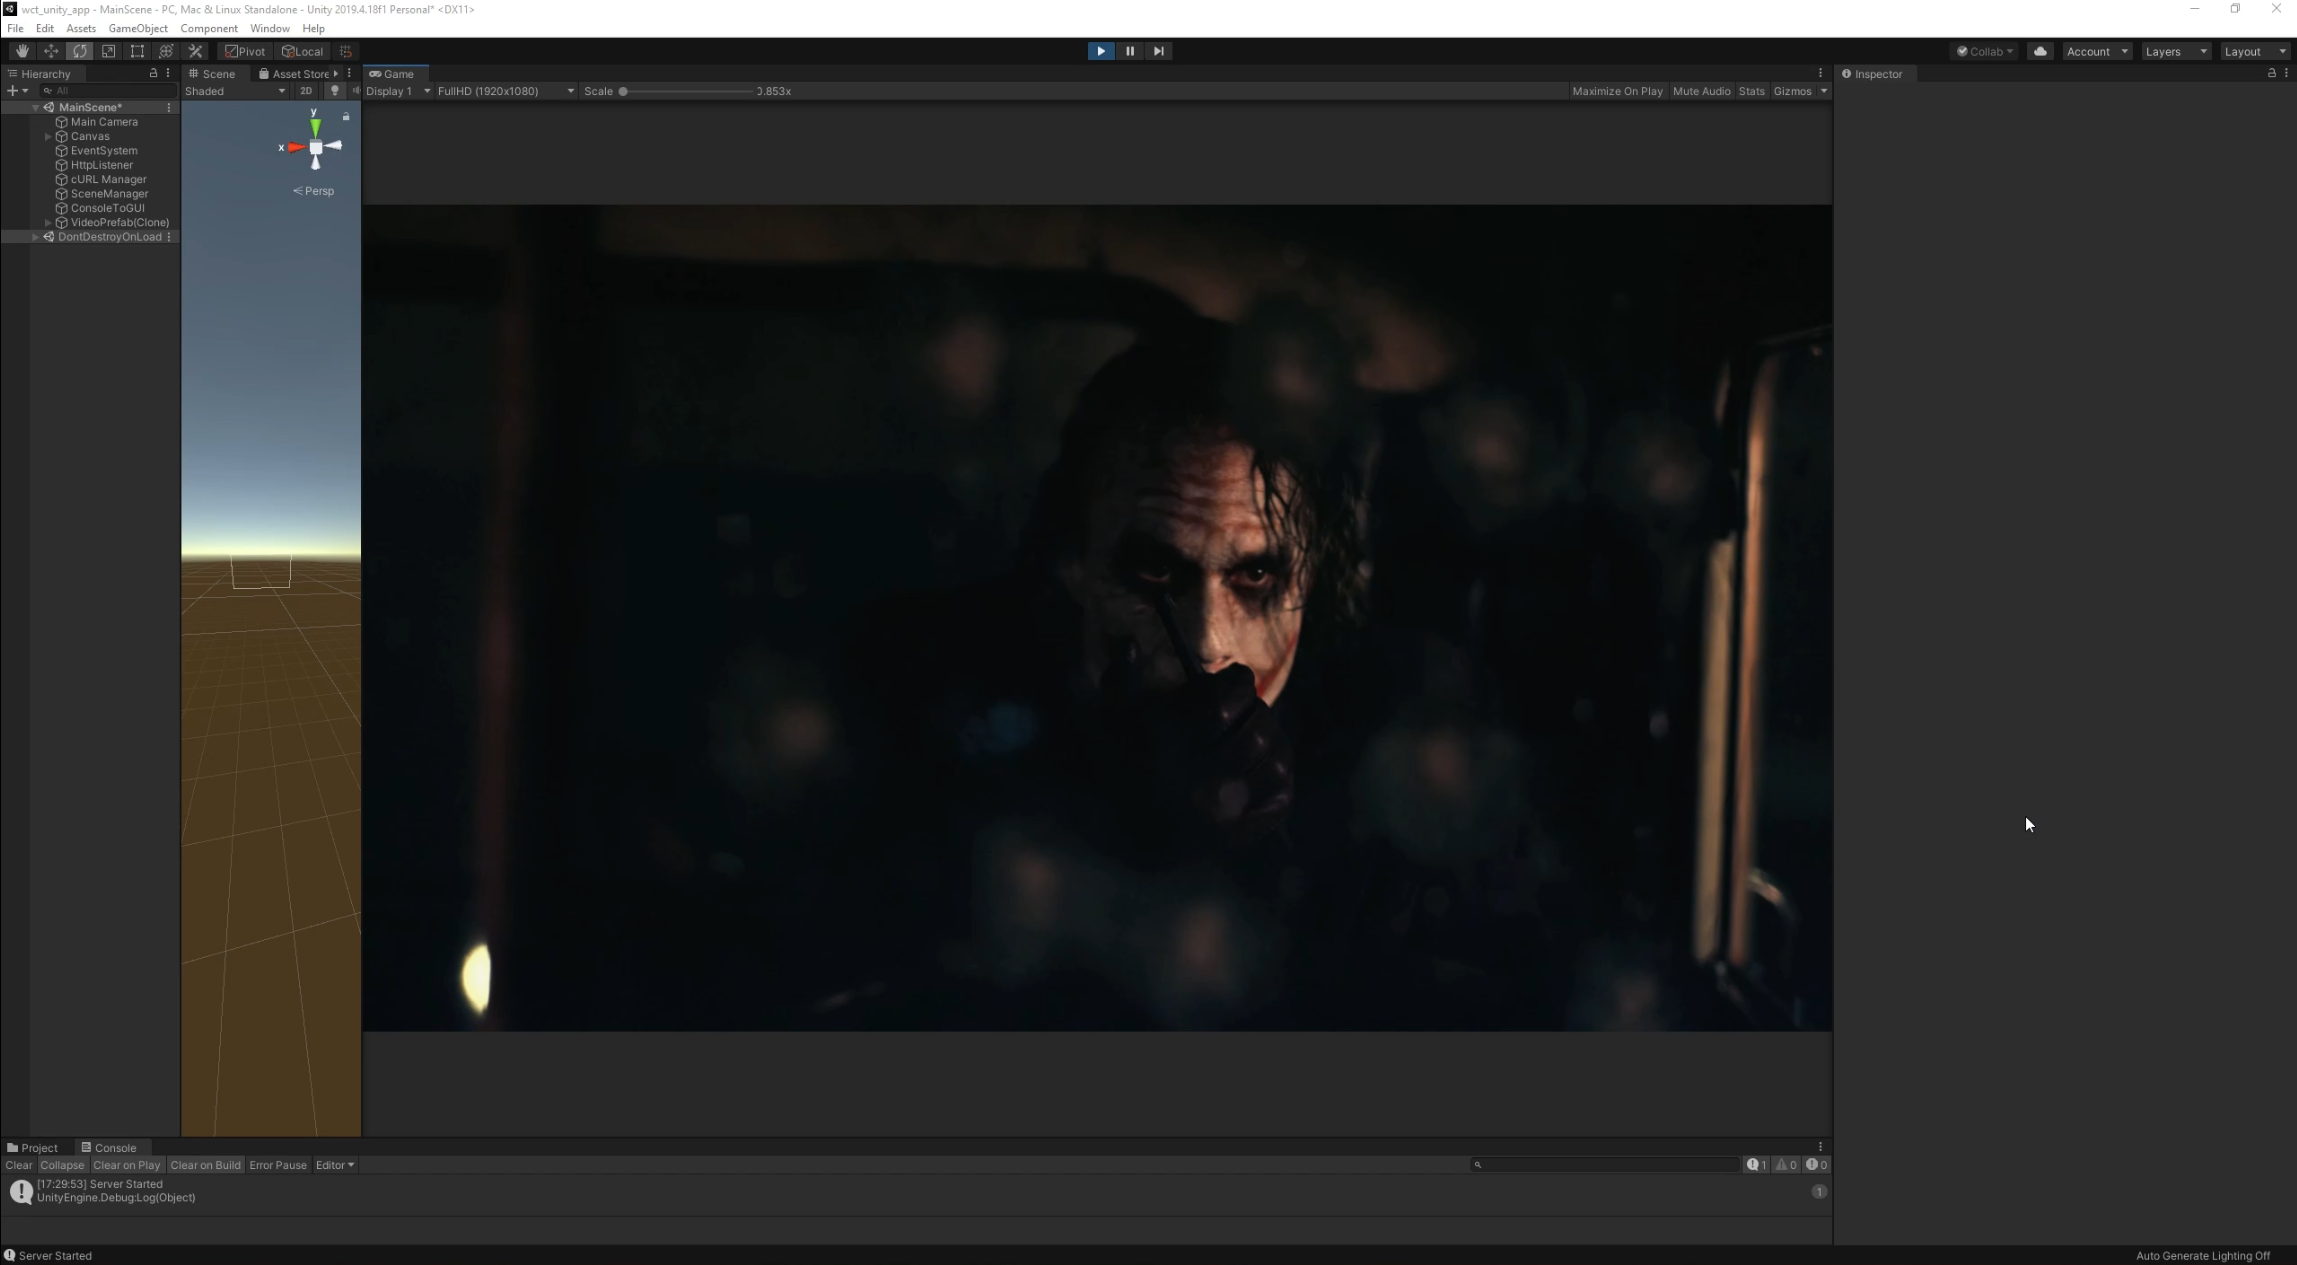
\includegraphics[height=7cm]{images/UMPvsAVPro}
\par\end{centering}
\caption{Prova UMP (Video 8K)\label{fig:UMPvsAVPro}}
\end{figure}

Les conclusions són que el AVPro és molt més potent per videos en
4K o més, pero en videos 1080p o menys, el rendiment és molt igualat,
i si tenim en compte que UMP accepta molts més formats, tenim un clar
guanyador pels objectius d'aquest projecte on resolucions de 4K o
més, no són la prioritat.\\

\subsubsection{Sortida del frame}

Per altre banda, la sortida del frame és més complicada, no és comú
voler treure per streaming el frame de Unity. La opció més viable
sembla utilitzar FFmpeg amb configuracions de piping. És a dir, hauriem
de generar les imatges a dins de Unity a una velocitat determinada
per aconseguir els FPS (Frames per second) desitjats. I després introduir-ho
a FFmpeg amb una comanda utilitzant <<pipe>> com a input.\\

Hi ha un projecte de Github \cite{FFmpegOut}, desenvolupat per l'usuari
Keijiro, molt conegut a la comunitat de Unity per crear una gran varietat
de plugins molt útils i innovadors. El que aconsegueix és introduir
FFmpeg a Unity, i utilitzar el mètode dels pipeline per grabar un
video local. Afortunadament el codi és open-source, pel que el podem
modificar per aconseguir que enlloc de generar un fitxer en local,
faci un streaming per rtp. Aconseguit això, ens trobem amb diversos
problemes. Amb Linux només suporta la API de render <<Vulkan>> \cite{Vulkan}.
És una API que està agafant molta força, però és millor evitar-la
ja que és encara molt nova, i el plugin de reproducció de video que
s'utilitza només suporta OpenGL. A part d'això i més important, l'àudio
no surt de cap manera, i s'ha de capturar de manera externa, pel que
serà molt complicat sincronitzar-ho amb el video.\\

Un altre opció és automatitzar unes comandes de FFmpeg per capturar
la finestra i generar un streaming de sortida. Com ja ha sigut comentat
abans, FFmpeg és l'eina més potent de video i es controla mitjançant
comandes al terminal, el que és molt útil per a poder automatitzar
les tasques a través de scripts.

\subsection{Elecció del hardware i sistema}

\subsubsection{Plataforma Virtual AWS}

L'elecció de la plataforma que contindrà el software no ha sigut gaire
complicada. Les opcions eren Azure, AWS (Amazon Web Services) \cite{AWS}
o Google. Es tracten de plataformes Cloud on es poden emmagatzemar
i executar tot tipus d'arxius. Són molt utilitzades ja que només les
mega corporacions disposen d'infraestructures de servidors propis,
la majoria de desenvolupadors lloguen els servidors a una d'aquestes
plataformes. Comparativa entre AWS i Azure \cite{AWSvsAzure}.

\begin{table}[H]
\begin{tabular}{|>{\centering}m{5.5cm}|>{\centering}m{5.5cm}|}
\hline 
\textbf{AWS} & \textbf{Azure}\tabularnewline
\hline 
Plataforma de computació al núvol sota demanda (Amazon) & Plataforma pública al núvol (Microsoft)\tabularnewline
\hline 
Amigable desde els seus inicis amb el model de codi obert & No tenen bona relació amb la comunitat de codi obert\tabularnewline
\hline 
Té una gran avantatge en quant a ofertes de núvol governamental & Limitat en quant a ofertes per al núovl governamental\tabularnewline
\hline 
Models de preu flexibles & Models de preus més tancats i menys varietat\tabularnewline
\hline 
Segueix donant recolzament per suportar els models de núvols híbrids & Excel·lent per models amb núvols hibrids\tabularnewline
\hline 
Gran varietat de software i sistemes operatius tant Linux com Windows & Està més limitat al sistema operatiu de Windows encara que també té
algunes opcions de Linux\tabularnewline
\hline 
El sistema d'emmagatzematge de AWS (EBS) és molt ràpid per sistemes
amb big data. & L'emmagatzematge estàndard té problemes amb el big data i per tant
s'ha de contractar un server de primera qualitat.\tabularnewline
\hline 
Entorns molt més madurs pel big data & Entorns més verds per big data, encara que Azure està millorant en
aquest aspecte\tabularnewline
\hline 
Es pot accedir a les màquines de manera individual & Les màquines estan agrupades en un sol servei al núvol i responen
al mateix domini però amb diferents ports\tabularnewline
\hline 
Elastic Compute Cloud (EC2) Es paga per hora utilitzada & Es paguen per minut\tabularnewline
\hline 
S3 Arxius de rcuperació a curt termini. Per llargs terminis es pot
utilitzar Glacier & Té una opció semblant a S3, però per recuperacions a llarg termini
encara no disposa de cap solució\tabularnewline
\hline 
La seguretat es proporciona a través de rols definits per l'usuari
administrador & Es defineix un director que serà l'administrador del servidor\tabularnewline
\hline 
\end{tabular}

\caption{Comparativa subjectiva de les possibles eines}
\end{table}

AWS és la millor opció per hostear aquest projecte, a més concorda
amb l'elecció de l'empresa on s'esta fent aquest projecte, Watchity,
que tenen tot el seu software i servidors contractats amb aquesta
plataforma.\\

\subsubsection{Sistema operatiu}

Per escollir el sistema operatiu més adient haurem de veure les ventatges
que té cada un dels més populars, que són: Windows, MacOS i Linux.
Tenint en compte que el projecte s'emmagatzemarà i s'executarà desde
un servidor de AWS, el més adient és tenir-ho amb el sistema operatiu
més popular al núvol, Linux. Windows també disposa d'opcions per ser
executat en un servidor, però les funcionalitats son infinitament
inferiors, a més de ser privatiu i no permetre la modificació de cap
element del sistema.\\

Per tant, sabent que el sistema operatiu serà Linux, també caldrà
escollir la distribució més adient. Les millors opcions són Ubuntu
Server, CentOS, SUSE i Arch. Cada un d'ells tenen les seves ventatges
i desventatges. A Watchity, treballen amb CentOS en totes les seves
màquines, ja que es una distribució molt sòlida i de les més utilitzades
per servidor. La diferència més gran entre aquests dos és que Ubuntu
al estar basat en Debian, els paquets són instalats en .deb amb el
gestor de paquets <<apt-get>>, mentres que a CentOS s'utilitza <<yum>>
o <<dnf>>.\\

Realment per aquest projecte és indiferent l'elecció d'un o un altre,
pel que s'escollirà CentOS simplement per no diferenciar-se a la metodologia
de treball de Watchity.

\begin{figure}[H]
\begin{centering}

\includegraphics[height=4cm]{images/CentOSLogo}
\par\end{centering}
\caption{CentOS Logo\label{fig:CentOS}}
\end{figure}

\section{Part Pràctica}

\subsection{Arquitectura del sistema}

L'aplicació es composarà d'un binari executable de Unity, emmagatzemat
a un servidor d'AWS. En aquest servidor es rebràn crides cURL a través
d'un frontend comprensible per l'usuari a qui va dirigit. Les peticions
dels usuaris seràn processades i <<traduïdes>> per fer els canvis
a l'aplicació de Unity d'una manera que entengui. El servidor estarà
emetent constantment la sortida del Unity amb un monitor virtual,
que serà enviada per multicast a la web on l'usuari està interactuant
per poder veure els canvis que ha realitzat.

\begin{figure}[H]
\begin{centering}
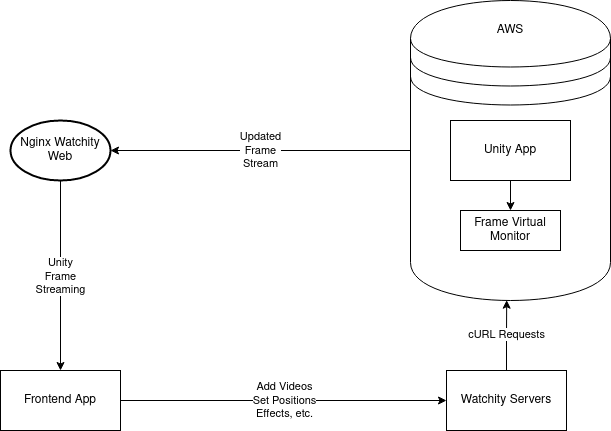
\includegraphics[height=7cm]{images/Arquitectura}
\par\end{centering}
\caption{Arquitectura del Projecte\label{fig:Arquitectura}}
\end{figure}

\subsection{Possibilitats}

\subsubsection{Resolució}

La resolució de l'aplicació serà per defecte 1920x1080. Això es defineix
a la configuració de la targeta gràfica del servidor d'AWS, concretament
a l'arxiu /etc/X11/xorg.conf. Aquest, és un arxiu de configuració
que utilitza Nvidia i que emmagatzema tot tipus de configuració gràfica,
ja sigui resolucions, tipus de targeta, monitors virtuals, refresc,
etc. Al tractar-se d'un servidor, les configuracions gràfiques s'han
de realitzar manualment, i crear un xorg.conf que s'adequï a les necessitats
de cada un. A continuació s'adjunta el fitxer xorg que s'ha realitzat
per aquest projecte.\\

\lstinputlisting[breaklines=true,captionpos=b,frame=tb,language=bash,caption={Configuració Gràfica | xorg.conf},label={Xorg}]{code/xorg.conf}

Començant amb la secció de <<Monitor>>, serveix per definir un nou
monitor, pel primer cas fem un primari amb el nom Monitor0, i en el
segon cas fem un monitor secundari amb el nom Monitor1, situat a l'esquerra
del primari. Aquest segon monitor es crea per si de cas en un futur
es volgués tenir més d'una aplicació de Unity executant-se a la vegada,
encara que la idea es tenir-ne només una en cada màquina AWS de forma
ordinària.\\

La següent secció és el <<Device>>, tracta de la targeta gràfica
que es té instalada, amb tota la informació necessaria, molt important
posar el model (Tesla T4), targetes molt potents que a disposició
de AWS, i el BusID, en aquest cas el PCI:0:30:0. Si no es posen aquestes
dades, podria no funcionar la conexió gràfica amb l'ordinador.\\

A la secció <<Screen>> es defineix la configuració de pantalla.
Molt diferent a la configuració de monitor. En aquest bloc es posarà
un nom identificador <<Screen0>>, el dispositiu gràfic que s'utilitza
<<Device0>> (referència a la GPU Nvidia Tesla T4), el monitor que
renderitza aquesta pantalla <<Monitor0>> la profunditat de color,
que són 24. Ja que utilitzarem el estàndard, corresponent al True
Color 24-bit, que utilitza 8-bits per cada color primari R, G i B.
Cada cop s'està utilitzant més el Deep Color que utilitza 10-bits
per canal, més conegut com a HDR (també existeix de 12-bits o més)
\cite{HDRGuia} en els televisors més actuals, si en volguéssim fer
ús i poder utilitzar contingut que disposi d'aquesta tecnologia hauriem
de posar un 30 en el valor de DefaultDepth. Però ara per ara, no interessa
utilitzar HDR i no és un objectiu proposat que l'aplicació ho permeti.

Seguit d'això es crea una subsecció que contindrà unes dades fixades
de com ha de ser la pantalla, amb una resolució de 1920x1080 i 24
de profunditat.

Per últim, i de manera opcional, es poden definir unes opcions de
comportament de la pantalla, el que s'ha utilitzat són les opcions
de ForceFullCompositionPipeline i TripleBuffer per evitar bugs gràfics
en els que la pantalla pot quedar tallada verticalment (un bug bastant
comú en sistemes Linux amb gràfiques d'Nvidia).

\begin{figure}[H]
\begin{centering}
\includegraphics[height=6cm]{images/VSyncXorg}
\par\end{centering}
\caption{Exemple Bug Gràfic VSync\label{fig:XorgVSync}}
\end{figure}

Vist això, queda provat que es pot definir qualsevol resolució al
sistema, nomes caldrà canviar l'arxiu de configuració xorg.conf i
posar la que es desitji. Es podria posar una resolució de 4K o 720p,
això si, lògicament com més alta sigui la resolució, més latència
es tindrà a la sortida.

\subsubsection{Compatibilitat fluxes d'entrada}

Per l'entrada de videos s'utilitza el plugin UMP de l'asset store
de Unity, que a la vegada aquest utilitza internament les llibreries
libVLC, pel que es permetrà qualsevol format que VLC accepti de manera
nativa. Segons la pròpia pàgina de Videolan, creadors de libVLC els
formats acceptats són:\\

\textbf{Vídeo Códecs}
\begin{itemize}
\item MPEG-1/2
\item DivX® (1/2/3/4/5/6)
\item MPEG-4 ASP
\item XviD
\item 3ivX D4
\item H.261
\item H.263 / H.263i, H.264 / MPEG-4 AVC
\item Cinepak
\item Theora
\item Dirac / VC-2
\item MJPEG (A/B)
\item WMV 1/2
\item WMV 3 / WMV-9 / VC-1
\item Sorenson 1/3
\item DV
\item On2 VP3/VP5/VP6
\item Indeo Video v3 (IV32)
\item Real Video (1/2/3/4)
\end{itemize}
%
\textbf{Àudio}
\begin{itemize}
\item MPEG Layer 1/2
\item MP3 - MPEG Layer 3
\item AAC - MPEG-4 part3
\item Vorbis
\item AC3 - A/52
\item E-AC-3
\item MLP / TrueHD>3
\item DTS
\item WMA 1/2
\item WMA 3
\item FLAC
\item ALAC
\item Speex
\item Musepack / MPC
\item ATRAC 3
\item Wavpack
\item Mod
\item TrueAudio
\item APE
\item Real Audio
\item Alaw/µlaw
\item AMR (3GPP)
\item MIDI
\item LPCM
\item ADPCM
\item QCELP
\item DV Audio
\item QDM2/QDMC
\item MACE
\end{itemize}
%
\textbf{Subtítols}
\begin{itemize}
\item DVD
\item Text files (MicroDVD, SubRIP, SubViewer, SSA1-5, SAMI, VPlayer)
\item Closed captions
\item Vobsub
\item Universal Subtitle Format (USF)
\item SVCD / CVD
\item DVB
\item OGM
\item CMML
\item Kate
\end{itemize}
%
\textbf{Fluxos d'entrada}
\begin{itemize}
\item UDP/RTP Unicast
\item UDP/RTP Multicast
\item HTTP / FTP
\item MMS
\item TCP/RTP Unicast
\item DCCP/RTP Unicast
\item Arxius Locals
\item DVD Video
\item Video CD / VCD
\item SVCD
\item Audio CD (no DTS-CD)
\item DVB (Satellite, Digital TV, Cable TV)
\item MPEG encoder
\item Video acquisition
\end{itemize}
%
\textbf{Formats d'entrada}
\begin{itemize}
\item MPEG (ES,PS,TS,PVA,MP3)
\item AVI
\item ASF / WMV / WMA
\item MP4 / MOV / 3GP
\item OGG / OGM / Annodex
\item Matroska (MKV)
\item Real
\item WAV (including DTS)
\item Raw Audio: DTS
\item AAC
\item AC3/A52
\item Raw DV
\item FLAC
\item FLV (Flash)
\item MXF
\item Nut
\item Standard MIDI / SMF
\item Creative™ Voice
\end{itemize}
%
En resum, tots els formats estandaritzats son perfectament compatibles
amb l'aplicació i hauria de ser bastant complicat trobar-se amb un
video incompatible per la reproducció.

\subsubsection{Control de l'app}

El control de l'aplicació es farà mitjançant comandes cURL, que contindran
text pla amb les instruccions que haurà de fer el Unity, per exemple
<<addVideo>>, <<destroyBackground>>, etc. La metodologia per utilitzar
cada funcionalitat serà semblant entre elles per aconseguir un ús
fluit i senzill d'entendre. Els elements estaràn separats en Videos,
Imatges, Textos i Background. Exceptuant el background, la resta seràn
un conjunt d'arrays ordenats per números, tindrem el video número
1, número 3, i no caldrà que tinguin un ordre seqüencial, a més de
crear arrays dinàmics per permetre una longitud infinita.

La metodologia de la comanda a seguir serà: 

\fontspec{FiraCode}
\begin{center}
{\fboxrule 0.2pt\fbox{\textsf{function=elementNumber\%attributes\textasciitilde optionalSettings}}}
\par\end{center}

\normalfont

Exemple:

\fontspec{FiraCode}
\begin{center}
{\fboxrule 0.2pt\fbox{addVideo=1\%/home/user/videoTest.mp4\textasciitilde 1}}
\par\end{center}

\normalfont

Seguint d'esquerra a dreta l'exemple que s'ha posat tenim a la banda
esquerra de l'igual, la funció que haurà de fer, en aquest cas addVideo,
és a dir, afegir un nou video a l'escena actual. Després de l'igual
tenim tots els atributs i configuració, en aquest cas posem el video
a la posició 1 (no posició espaial, sinó de l'array), utilitzem el
separador \% per introduir l'atribut principal que pràcticament totes
les funcionalitats tindran, per aquest exemple serà la ruta on es
trova el video que es vol reproduir.

\subsubsection{Compatibilitat audio}

Per altre banda tenim el sistema d'àudio, en el que un usuari pot
posar una cancó, veu en off, o el que vulgui de fons. Aquí no s'utilitza
libVLC, sinó la llibreria interna d'àudio de la que disposa Unity,
pel que serà compatible únicament amb audio WAV i MPEG, que ha de
ser més que suficient tenint en compte que no és un objectiu principal
ni molt demandat, i es compleix un suport dels estandards d'àudio.
Això sí, s'accepten fitxers tant locals com al núvol, descarregant
la informació d'aquests, i emmagatzemant-la en un array d'AudioClips.\\

\lstinputlisting[breaklines=true,captionpos=b,frame=tb,language={[Sharp]C},caption={Àudio | addAudio.cs},label={AddAudio}]{code/unityCode/addAudio.txt}

\subsubsection{Transicions}

Es permeten 3 tipus de transicions en videos, per tall, crossfade
i fade. En la de tall, passem d'un video a un altre d'una manera brusca.
El crossfade significa canviar d'un video a un altre fent que un va
desapareixent mentres el segon apareix, pel que no passem per un pla
en negre i pot quedar més dinàmic segons el moment. En el fade en
canvi, el primer video es va difuminant fins a passar a un pla en
negre, i un cop s'ha arribat al negre, el segon apareix de manera
gradual.\\

Per fer ús d'aquestes funcionalitats disposarem de 2 comandes:\\

\lstinline!dissolve="videoNumber%link_or_local_path"!

\pagebreak{}
\begin{thebibliography}{10}
\bibitem{ControlRoom}Watchity. (2019b, September 13). ¿Qué es el
Control Room (Live Distribution)? Watchity - Help Center. https://help.watchity.com/hc/es/articles/360017584293-{}-Qu\%C3\%A9-es-el-Control-Room-Live-Distribution-

\bibitem{Cut=000026Share}Watchity. (2020, July 8). Share cuts on
Social Networks. Watchity - Help Center. https://help.watchity.com/hc/en-us/articles/360023619094-Share-cuts-on-Social-Networks

\bibitem{Mixer}Watchity. (2019, September 9). ¿Qué es el Mixer? Watchity
- Help Center. https://help.watchity.com/hc/es/articles/360018866273-{}-Qu\%C3\%A9-es-el-Mixer-

\bibitem{HeadlessChromeExp1}Pereyro, S. (2018, February 09). Live
streaming with headless chrome - Empirical. Empirical. https://blog.goempirical.com/how-to-use-headless-chrome-to-screencast-audio-and-video-to-an-rtmp-endpoint-216ccfdde4db

\bibitem{PulseAudio}FreeDesktop. (2021, January 16). PulseAudio.
https://www.freedesktop.org/wiki/Software/PulseAudio/

\bibitem{HeadlessChromeDevel}Google. (2021, February 25). Getting
Started with Headless Chrome | Web |. Google Developers. https://developers.google.com/web/updates/2017/04/headless-chrome

\bibitem{Selenium}SeleniumHQ. (2018, December 19). SeleniumHQ Browser
Automation. Selenium. https://www.selenium.dev/

\bibitem{SeleniumDriverDocumentation}SeleniumHQ. (2021a, July 7).
Driver requirements :: Documentation for Selenium. Documentació Selenium.
https://www.selenium.dev/documentation/en/webdriver/driver\_requirements/

\bibitem{SeleniumHeadlessChrome}Smirnov, A. (2020, November 18).
How to run a headless Chrome browser in Selenium WebDriver. Medium.
https://itnext.io/how-to-run-a-headless-chrome-browser-in-selenium-webdriver-c5521bc12bf0

\bibitem{Puppeteer}Google. (2021a, February 11). Puppeteer | Tools
for Web Developers |. Google Developers. https://developers.google.com/web/tools/puppeteer

\bibitem{ApacheLicense}Apache. (2004, January 1). Apache License,
Version 2.0. Apache License. https://www.apache.org/licenses/LICENSE-2.0

\bibitem{WebGLBrowserSupport}Mozilla. (2021, May 27). WebGL: 2D and
3D graphics for the web - Web APIs | MDN. WebGL Support by Browser.
https://developer.mozilla.org/en-US/docs/Web/API/WebGL\_API\#browser\_compatibility

\bibitem{UE4BestPhotoEngine}Dealessandri, M. (2020, May 14). What
is the best game engine: is Unreal Engine right for you? GamesIndustry.Biz.
https://www.gamesindustry.biz/articles/2020-01-16-what-is-the-best-game-engine-is-unreal-engine-4-the-right-game-engine-for-you

\bibitem{PopularUnity}Eric Peckham, E. P. (2019, October 17). TechCrunch
is now a part of Verizon Media. Extra Crunch. https://techcrunch.com/2019/10/17/how-unity-built-the-worlds-most-popular-game-engine/

\bibitem{UnityMultiplatform}Technologies, U. (2021, January 1). Multiplatform.
Unity. https://unity.com/features/multiplatform

\bibitem{TIOBE}TIOBE. (2021, July 1). index | TIOBE - The Software
Quality Company. https://www.tiobe.com/tiobe-index/

\bibitem{MonoBehaviour}Technologies, U. (2021b, January 1). Unity
- Scripting API: MonoBehaviour. Unity. https://docs.unity3d.com/ScriptReference/MonoBehaviour.html

\bibitem{HDRP}Lagarde, S. (2020, February 24). HDRP: Out of Preview
in 2019.3. Unity Blog. https://blog.unity.com/technology/hdrp-out-of-preview-in-2019-3

\bibitem{DivX}Texto: Luz Fernández. (2002, December 28). La copia
de películas se hace fácil en Internet. Cinco Días. https://cincodias.elpais.com/cincodias/2002/12/28/tecnologia/1041322677\_850215.html

\bibitem{StreamingProtocols}Bychok, A. (2021, May 21). Streaming
Protocol Comparison: RTMP, WebRTC, FTL, SRT -- Restream Blog. Ultimate
Live Streaming Hub -- Restream Blog. https://restream.io/blog/streaming-protocols/

\bibitem{AV1Codec}Fernández, Y. (2019, November 7). Qué es el códec
AV1 y cuáles son sus ventajas. Xataka. https://www.xataka.com/basics/que-codec-av1-cuales-sus-ventajas

\bibitem{MixerFTL}Hao, D. T. G. (2019, August 7). Mixer’s Faster
Than Light streaming protocol explained. Dot Esports. https://dotesports.com/streaming/news/mixers-faster-than-light-streaming-protocol-explained

\bibitem{MixerCierre}Rus, C. (2020, June 23). Microsoft cierra Mixer,
su alternativa a Twitch en la que tenía en exclusiva a superestrellas
de eSports como. . . Xataka. https://www.xataka.com/videojuegos/microsoft-cierra-mixer-su-alternativa-a-twitch-que-tenia-exclusiva-a-superestrellas-esports-como-ninja

\bibitem{TwtichRTMP}Twitch. (2015, December 18). Twitch Blog | Twitch
Engineering: An Introduction and Overview. Twitch Blog. https://blog.twitch.tv/en/2015/12/18/twitch-engineering-an-introduction-and-overview-a23917b71a25/

\bibitem{FFmpeg About}FFmpeg. (2021, January 1). About FFmpeg. https://ffmpeg.org/about.html

\bibitem{FFmpeg Filters}FFmpeg. (2021b, January 1). FFmpeg Filters
Documentation. https://ffmpeg.org/ffmpeg-filters.html

\bibitem{VideoLAN}VideoLAN. (2021, January 1). Free Software and
Open Source video streaming solution for every OS! - VideoLAN. https://www.videolan.org/videolan/

\bibitem{VideoLAN Contribution}VideoLAN. (2021a, January 1). Contribute
to the project - VideoLAN. https://www.videolan.org/contribute.html

\bibitem{libVLCSampleCode}VideoLAN. (2019, March 4). libVLC Tutorial
- VideoLAN Wiki. WikiVLC. https://wiki.videolan.org/LibVLC\_Tutorial/

\bibitem{HeadlessChromeProject}Pereyro, S. (2017, October 31). Screencast
with Headless Chrome. Google Docs. https://docs.google.com/presentation/d/1b-HvxKmeFYE3qoNDJDHfbgVwEbi0QgmTvpH8w4CK5Tw/edit\#slide=id.gc6f90357f\_0\_0

\bibitem{Postman}Postman. (2021, January 1). Postman | The Collaboration
Platform for API Development. https://www.postman.com/

\bibitem{ChromeDevTools}Google. (2021a, January 1). Chrome DevTools
Protocol. Page Domain. https://chromedevtools.github.io/devtools-protocol/tot/Page/\#method-startScreencast

\bibitem{Nightcrawler}Filmaffinity. (2014, January 1). Nightcrawler
(2014). https://www.filmaffinity.com/es/film779937.html

\bibitem{Stalker}Filmaffinity. (1979, January 1). Stalker (1979).
https://www.filmaffinity.com/es/film534365.html

\bibitem{AutoplayPolicy}Google. (2017, September 13). Autoplay policy
in Chrome. Chrome Developers. https://developer.chrome.com/blog/autoplay/

\bibitem{FFmpegPatternType}FFmpeg. (2021c, January 1). FFmpeg Formats
Documentation. https://ffmpeg.org/ffmpeg-formats.html\#image2-1

\bibitem{FBSamplesRepo}FBSamples. (2020, May 8). GitHub - fbsamples/Canvas-Streaming-Example:
This project contains example code showing how to go live on Facebook
using a element as a source. GitHub. https://github.com/fbsamples/Canvas-Streaming-Example

\bibitem{NewTekNDI}NewTek. (2021, January 1). About NDI - Network
Device Interface. https://www.ndi.tv/about-ndi/

\bibitem{NDI Unreal Documentation}NewTek. (2020, November). NDI Unreal
Documentation. NDI Unreal Documentation. http://514f211588de67e4fdcf-437b8dd50f60b69cf0974b538e50585b.r63.cf1.rackcdn.com/Utilities/SDK/NDI\_SDK\_Unreal\_Engine/4.25/NDI\%20IO\%20Plugin\%20for\%20Unreal\%20Engine\%20Quickstart\%20Guide.pdf

\bibitem{UMP Plugin}Unity Direction Kit. (2016, June 4). UMP (Win,
Mac, Linux, WebGL) | Video. Unity Asset Store. https://assetstore.unity.com/packages/tools/video/ump-win-mac-linux-webgl-49625

\bibitem{Cloud Linux}Verma, A. (2015, August 30). Access denied |
fossbytes.com used Cloudflare to restrict access. Fossbytes. https://fossbytes.com/ubuntu-linux-is-the-most-popular-operating-system-in-cloud/

\bibitem{AVPro}RenderHeadsLTD. (2020, March 12). AVPro Video - Ultra
Edition | Video. Unity Asset Store. https://assetstore.unity.com/packages/tools/video/avpro-video-ultra-edition-184294

\bibitem{FFmpegOut}Keijiro, K. (2019, October 24). GitHub - keijiro/FFmpegOut:
Video capture plugin for Unity with FFmpeg. GitHub. https://github.com/keijiro/FFmpegOut

\bibitem{Vulkan}AMD. (2016, February 16). Vulkan. https://www.amd.com/es/technologies/vulkan

\bibitem{AWS}Amazon. (2021, January 1). AWS | Cloud Computing - Servicios
de informática en la nube. Amazon Web Services, Inc. https://aws.amazon.com/es/

\bibitem{AWSvsAzure}AWS vs Azure-Who is the big winner in the cloud
war? (2021, July 27). ProjectPro. https://www.dezyre.com/article/aws-vs-azure-who-is-the-big-winner-in-the-cloud-war/401

\bibitem{HDRGuia}López, J. C. (2019, February 20). La biblia del
HDR: qué es, cuáles son los estándares actuales y cómo no todo lo
que dicen que es HDR lo es en. . . Xataka. https://www.xataka.com/televisores/biblia-hdr-que-cuales-estandares-actuales-como-no-todo-que-dicen-que-hdr-efectivamente
\end{thebibliography}
\section{Images References}

\ref{fig:Frontend-Mixer} Watchity. (2019, September 9). Frontend
Mixer {[}Graph{]}. Frontend Mixer. https://help.watchity.com/hc/article\_attachments/360027399494/Tipo\_Production.png

\ref{fig:Selenium-Graph} SeleniumHQ. (2021, July 7). Selenium Driver
Graph {[}Graph{]}. Selenium Driver Graph. https://www.selenium.dev/documentation/images/basic\_comms.png?width=400px

\ref{fig:PupeteerLogo} pupeteer. (2018, January 12). Pupeteer Logo
{[}Graph{]}. Logo. https://user-images.githubusercontent.com/10379601/29446482-04f7036a-841f-11e7-9872-91d1fc2ea683.png

\ref{fig:WebGLExample} WebGL Example. (2017, March 17). {[}Illustration{]}.
Aquarium. https://1stwebdesigner.com/wp-content/uploads/2014/03/aquarium.png

\ref{fig:QuixelMegascans} Quixel. (2019, March 20). Quixel Megascan
{[}Render{]}. UE4 Demo. https://www.youtube.com/watch?v=9fC20NWhx4s

\ref{fig:BlueprintRotate} Spiris, S. (2014, December 25). Blueprint
{[}Graph{]}. UE4 Simple Blueprint. https://answers.unrealengine.com/storage/temp/24917-rotate90degrees.png

\ref{fig:BlueprintChaos} Neginfinity, N. (2013, January 27). Chaos
Blueprint {[}Graph{]}. UE4 Blueprint Example of Bad Node Programming.
https://forum.unity.com/proxy.php?image=https\%3A\%2F\%2Fpbs.twimg.com\%2Fmedia\%2FDeiyJrDUwAAJQJ8.jpg\&hash=f36b58c4bd4dc432a0a0ff8c62b453c4

\ref{fig:TiobeRanking} Daria, D. (2021, July 12). Ranking Languages
2020 {[}Graph{]}. Darly Solutions. https://darly.solutions/the-most-popular-programming-languages-in-2021/

\ref{fig:BookOfDead} Unity. (2018, January 16). Book of the Dead
- Unity Interactive Demo - Teaser. YouTube. https://www.youtube.com/watch?v=DDsRfbfnC\_A

\ref{fig:EFTCaptura} BATTLESTATE GAMES LIMITED. (2015, December 22).
Pantalla de Pre-Alfa 19. www.escapesfromtarkov.com. https://www.escapefromtarkov.com/media/id/29?lang=es

\ref{fig:DiagramaProtocol} Aakanksha, A. (2016, May 12). Diagrama
Protocol-Format-Códec {[}Graph{]}. StreamShark. https://streamshark.io/blog/understanding-codecs-and-formats/

\ref{fig:TCPvsUDP} Ruether, T. (2021, March 16). TCP vs UDP {[}Graph{]}.
Wowza. https://www.wowza.com/wp-content/uploads/Graphic-UDP-Vs-TCP-Diagram\_1150x685.webp

\ref{fig:LatencyGraph} Ruether, T. (2021a, March 16). Graph Latency
Streaming Protocols {[}Graph{]}. Wowza. https://www.wowza.com/wp-content/uploads/latency-continuum-2021-with-protocols-700x300-1.webp

\ref{fig:FFmpeg} FFmpeg. (2013, April 10). FFmpeg Logo {[}Logo{]}.
Wikipedia Media. https://upload.wikimedia.org/wikipedia/commons/thumb/5/5f/FFmpeg\_Logo\_new.svg/1280px-FFmpeg\_Logo\_new.svg.png

\ref{fig:VLC1} Brinkmann, M. (2009, July 7). VLC 1.0 {[}Photograph{]}.
Ghacks.Net. https://www.ghacks.net/2009/07/07/vlc-media-player-1-0-released/

\ref{fig:ExperimentHCEmpirical} Pereyro, S. (2017, October 31). Screencast
with Headless Chrome. Google Docs. https://docs.google.com/presentation/d/1b-HvxKmeFYE3qoNDJDHfbgVwEbi0QgmTvpH8w4CK5Tw/edit\#slide=id.gc6f90357f\_0\_0

\ref{fig:HCTestindexhtml} Vicente A. (2021, March 9) Test Headless
Chrome Index. Own elaboration.

\ref{fig:NDIVLC} NewTek. (2016, August 31). NDI VLC Output Config
{[}Config{]}. NewTek. https://www.newtek.com/blog/tips/vlc-media-player-and-newtek-ndi-vlc-plugin/

\ref{fig:NDIReceiver} NewTek. (2020b, November 20). NDI Receiver
Unreal {[}Graph{]}. NewTek. https://encrypted-tbn0.gstatic.com/images?q=tbn:ANd9GcRMEVIL0BGn1XzKBxR2VKpZowQagdDYYENRmA\&usqp=CAU

\ref{fig:NDIReceiverResultat} Vicente A. (2021, June 1) Test NDI
Receiver. Own elaboration.

\ref{fig:UMPFunctions} Unity Direction Kit. (2016a, June 4). UMP
Functionalities {[}Graph{]}. Asset Store. https://assetstorev1-prd-cdn.unity3d.com/key-image/9f96a930-72d3-4972-a650-f4ea4f6e326b.webp

\ref{fig:ProvaUnity} Vicente A. (2021, January 14) Test Unity UMP.
Own elaboration.

\ref{fig:AVProvsUMP} Vicente A. (2021, March 25) Test AVPro vs UMP.
Own elaboration.

\ref{fig:UMPvsAVPro} Vicente A. (2021, March 25) Test UMP vs AVPro.
Own elaboration.

\ref{fig:CentOS} CentOS. (2015, December 12). CentOS {[}Logo{]}.
Wiki. https://upload.wikimedia.org/wikipedia/commons/thumb/b/bf/Centos-logo-light.svg/658px-Centos-logo-light.svg.png

\ref{fig:Arquitectura} Vicente A. (2021, January 18) Esquema Arquitectura.
Own elaboration.

\ref{fig:XorgVSync} Vicente A. (2021, January 18) Exemple Bug Gràfic
VSync. Own elaboration (clip is from Kingsman 2014).

\section{Annexes}

\end{document}
\end{document}
